%testing git
\listfiles
\documentclass[manuscript, screen]{acmart} %review
%\setcitestyle{super,sort&compress}
\citestyle{acmauthoryear}
\usepackage{booktabs} % For formal tables
\usepackage{amssymb}
\usepackage{amsmath}

\usepackage[ruled]{algorithm2e} % For algorithms
\usepackage[caption = true]{subfig} % For subfigures
\usepackage[export]{adjustbox}
\usepackage{caption}
\usepackage{multirow}

% Metadata Information
\acmJournal{CIE}
\acmVolume{9}
\acmNumber{4}
\acmArticle{39}
\acmYear{2017}
\acmMonth{12}

%\acmBadgeL[http://ctuning.org/ae/ppopp2016.html]{ae-logo}
%\acmBadgeR[http://ctuning.org/ae/ppopp2016.html]{ae-logo}

% Copyright
\setcopyright{acmcopyright}
%\setcopyright{acmlicensed}
%\setcopyright{rightsretained}
%\setcopyright{usgov}
%\setcopyright{usgovmixed}
%\setcopyright{cagov}
%\setcopyright{cagovmixed}

% DOI
\acmDOI{0000001.0000001}


% Document starts
\begin{document}
% Title portion
\title{A Unified Model for the Mobile-Edge-Cloud Computational Continuum} 
 %\titlenote{This is a titlenote}
 %\subtitle{This is a subtitle}
 %\subtitlenote{Subtitle note}

%\author{Gang Zhou}
%\orcid{1234-5678-9012-3456}
%\affiliation{%
%  \institution{College of William and Mary}
%  \streetaddress{104 Jamestown Rd}
%  \city{Williamsburg}
%  \state{VA}
%  \postcode{23185}
%  \country{USA}}
%\email{gang_zhou@wm.edu}
%\author{Valerie B\'eranger}
%\affiliation{%
%  \institution{Inria Paris-Rocquencourt}
%  \city{Rocquencourt}
%  \country{France}
%}
%\email{beranger@inria.fr}
%\author{Aparna Patel} 
%\affiliation{%
% \institution{Rajiv Gandhi University}
% \streetaddress{Rono-Hills}
% \city{Doimukh} 
% \state{Arunachal Pradesh}
% \country{India}}
%\email{aprna_patel@rguhs.ac.in}
%\author{Huifen Chan}
%\affiliation{%
%  \institution{Tsinghua University}
%  \streetaddress{30 Shuangqing Rd}
%  \city{Haidian Qu} 
%  \state{Beijing Shi}
%  \country{China}
%}
%\email{chan0345@tsinghua.edu.cn}
%\author{Ting Yan}
%\affiliation{%
%  \institution{Eaton Innovation Center}
%  \city{Prague}
%  \country{Czech Republic}}
%\email{yanting02@gmail.com}
%\author{Tian He}
%\affiliation{%
%  \institution{University of Virginia}
%  \department{School of Engineering}
%  \city{Charlottesville}
%  \state{VA}
%  \postcode{22903}
%  \country{USA}
%}
%\affiliation{%
%  \institution{University of Minnesota}
%  \country{USA}}
%\email{tinghe@uva.edu}
\author{Author 1}
\author{Author 2}
\author{Author 3}
\author{Author 4}
\affiliation{%
  \institution{Politecnico di Milano}
  \department{Dipartimento di Elettronica, Informazione e Bioingegneria }
  \city{Milan}
  \state{MI}
  \postcode{20133}
  \country{Italy}
}

\renewcommand\shortauthors{Zhou, G. et al}

\begin{abstract}
%Multifrequency media access control has been well understood in
general wireless ad hoc networks, while in wireless sensor networks,
researchers still focus on single frequency solutions. In wireless
sensor networks, each device is typically equipped with a single
radio transceiver and applications adopt much smaller packet sizes
compared to those in general wireless ad hoc networks. Hence, the
multifrequency MAC protocols proposed for general wireless ad hoc
networks are not suitable for wireless sensor network applications,
which we further demonstrate through our simulation experiments. In
this article, we propose MMSN, which takes advantage of
multifrequency availability while, at the same time, takes into
consideration the restrictions of wireless sensor networks. Through
extensive experiments, MMSN exhibits the prominent ability to utilize
parallel transmissions among neighboring nodes. When multiple physical
frequencies are available, it also achieves increased energy
efficiency, demonstrating the ability to work against radio
interference and the tolerance to a wide range of measured time
synchronization errors.\footnote{This is an abstract footnote}
\end{abstract}


%
% The code below should be generated by the tool at
% http://dl.acm.org/ccs.cfm
% Please copy and paste the code instead of the example below. 
%
\begin{CCSXML}
<ccs2012>
<concept>
<concept_id>10010520.10010521.10010537.10010538</concept_id>
<concept_desc>Computer systems organization~Client-server architectures</concept_desc>
<concept_significance>500</concept_significance>
</concept>
<concept>
<concept_id>10010520.10010570.10010573</concept_id>
<concept_desc>Computer systems organization~Real-time system specification</concept_desc>
<concept_significance>500</concept_significance>
</concept>
<concept>
<concept_id>10010520.10010570.10010574</concept_id>
<concept_desc>Computer systems organization~Real-time system architecture</concept_desc>
<concept_significance>500</concept_significance>
</concept>
<concept>
<concept_id>10010520.10010521.10010537.10003100</concept_id>
<concept_desc>Computer systems organization~Cloud computing</concept_desc>
<concept_significance>300</concept_significance>
</concept>
</ccs2012>
\end{CCSXML}

\ccsdesc[500]{Computer systems organization~Client-server architectures}
\ccsdesc[500]{Computer systems organization~Real-time system specification}
\ccsdesc[500]{Computer systems organization~Real-time system architecture}
\ccsdesc[300]{Computer systems organization~Cloud computing}

%
% End generated code
%


\keywords{Edge computing, Cloud computing, low-latency applications, mobile computation offloading, serverless computing}


\maketitle


\section{Introduction}

%What: The need of edge computing to enable low latency and mobile computation offloading
\subsubsection*{Problem Statement}

With the advent of Internet of Things, the evolution of mobile computing, and the emergence of real-time applications, the processing of an exponentially increasing volume of data must be performed in a timely fashion, i.e., with minimum latency. Despite the elasticity and vast computing power of existing cloud platforms, the access to these resources involves multiple hops of network communication, adding prohibitive latency to requests' processing. Such limitation has the following implications:

\begin{enumerate}

\item Cloud services may fail to satisfy the requirements of real-time and low-latency client applications; and

\item Offloading of delay-sensitive computation from devices with constrained resources to cloud servers is unlikely to work due to network-latency.

\end{enumerate}

%What: The challenges in realizing edge computing
\subsubsection*{Edge Computing}

To reduce network latency, data processing must be performed closer to where it is produced and consumed. In accordance with this principle, the emerging paradigm of edge computing~\cite{} states that computing power should be pushed from centralized datacenters to the edge of the network. 
%What: The challenges in the realization of edge computing
The realization of this paradigm, however, still poses many challenges:

%What: Resouce limitations of edge computing

--- First, a highly distributed edge infrastructure is not expected to exhibit virtually unlimited resources as cloud datacenters. This limitation requires a more efficient allocation of edge resources. Current models based on virtualization and containerization, although successfully adopted by cloud providers, may not be feasible in the context of edge computing.

%What: Aways availability does not work

--- Second, cloud services cover very large areas in which requests from clients are always expected. In contrast, edge infrastructure features a fine-grained coverage area~\cite{Dehos14millimeter5g} where edge services would remain idle whenever clients are absent in their coverage area. Therefore, to optimize the usage of edge resources, it should support the opportunistic deployment of services.

%What: The need for taking alternative edge domains into account

--- Third, different types of edge computing infrastructure may exist, including servers located at cellular base stations, temporarily placed nearby public events, and inside buildings and houses to provide support for smart spaces applications. The eventual co-existence of edge alternatives would require the client-side participation on the decision of which alternative to use.

%What: The need for a single model for the computing continuum

\subsubsection*{Compute Continuum}

Considering a high availability and elasticity of cloud-based services and an opportunistic nature of edge-based services that may not always be available, the later should complement rather than replace the former. This vision also extends to the computation that may opportunistically be offloaded from resource constrained mobile devices to nearby edge servers. In this sense, cloud, edge, and mobile computing should be seen as a \textit{compute continuum}, as depicted in Figure~\ref{fig:continuum}. Its materialization requires not only the realization of edge computing, but also a model that allows computation to be seamlessly displaced from one part of the continuum to the other depending on the context. 

\begin{figure}[tbp]
	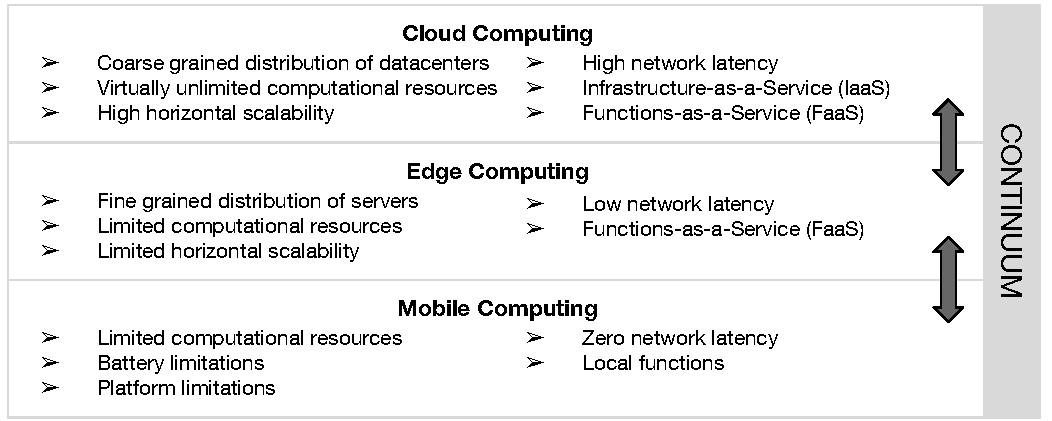
\includegraphics[width=0.9\textwidth]{figs/Continuum.pdf}
	\caption{Compute continuum formed by Cloud, Edge, and Mobile Computing}
	\label{fig:continuum}
\end{figure}
 

%--- Last but not least, cloud servers should not be disregarded as a part of the Cloud-to-Edge continuum. %not sure whether to call it Cloud-to-Things or Cloud-to-Edge
%First, because client applications may still rely on Cloud backends for traditional, non delay-sensitive computation. Second, because edge servers may be unavailable from the certain locations. Thus, client applications must rely on a runtime mechanism to discover and negotiate the use of nearby edge infrastructure. As the alternative infrastructures (including the cloud) may exhibit uneven loads in different moments, the decision of which to use, must take into account their current status as well as the client application requirements in terms of latency and computational power. 


%Finally, to avoid increasing the burden of application development, computation to be executed at the edge should follow, to the extent possible, a common architecture and implementation with respect to its cloud counterpart. The same applies to the computation that may be offloaded from resource constrained devices to nearby edge infrastructure.  

%\subsection{Serverless Computing}

%Serverless computing~\cite{Roberts:2016, Hendrickson:2016}, also known as Functions-as-a-Service (FaaS)~\cite{MateosFaaster17}, emerged as an alternative execution model within cloud computing. In particular, its name derives from the fact that server management and capacity planning decisions are hidden from the software application engineers. Instead, third party providers of the serverless platform dynamically manage resource allocation and sharing for the execution of different types of computational tasks, known as \textit{functions}. Nowadays, all major cloud vendors provide serverless runtimes an associated ecosystem of services. 
%
%Among its main advantages, the serverless model is cost- and resource-efficient in comparison to virtual machine and container-based provisioning models, which generally involve significant periods of underutilization or idle time. In previous work~\cite{GarrigaMendonca2017}, we discussed the suitability of a serverless architecture to enable low-latency applications to use edge computing computational resources in an efficient, scalable and automated way. In this work, serverless computing is further explored in the realization of the compute continuum composed also by cloud and mobile devices by means of a unified model.

%mobile devices could make use of compute runtimes deployed at nearby edge servers to extend their capabilities. Notwithstanding the potential of such combination, a complete model for its realization is still missing~\cite{NasticServerlessEdge17}. 

\subsubsection*{Contributions of this Work}

%What: A3-E model (process?) as a contribution

In this paper, we propose A3-E --- \textit{(A)wareness, (A)cquisition, (A)llocation and (E)ngagement} --- a unified model that empowers applications to leverage the computing continuum formed by cloud, edge, and mobile computing. A3-E processes encompasses different phases and activities to be performed whether by servers or clients. Also, different instances of the process may apply to variations of cloud, edge, and local computing.

%What: A3-E and Serverless Computing 

In accordance with our previous work~\cite{GarrigaMendonca2017}, A3-E embraces the paradigm serverless computing~\cite{Hendrickson:2016,baldini2017serverless} in the realization of the continuum. In specific, A3-E explores the function-as-a-service (FaaS) model~\cite{MateosFaaster17} to allow stateless functions to be quickly deployed and exposed as services, providing an efficient and scalable allocation of computing resources that fits well with the resource limitations of edge computing. A3-E further extends FaaS with the complete automation of services life-cycle, including the deployment of services by servers. Such an autonomy releases developers and administrators from the burden of deployment and maintenance, and further supports the materialization of a fine-grained distribution of the network edge and the continuum as a whole.

%What: The obtained results for latency and battery; other metrics?

As demonstrated through different experiments, an AR application could rely on services dynamically selected and implemented as functions that are executable locally, in the edge, or in the cloud. The experiments have shown a XX\% reduction of latency when edge services were used instead of cloud services, and a YY\% decrease of battery consumption when computation was offloaded from the mobile device to nearby edge server. These results corroborates the importance of edge computing and the feasibility of A3-E in realizing the cloud-edge-mobile continuum.

%Finally, experiments with an augmented reality application have also shown the feasibility of A3-E model in the realization of the continuum, with a single client application been able to seamlessly alternate among local, edge, and cloud-based services.

% Such a selection is performed according to the application requirements (e.g., latency) and the actual context of the continuum as perceived by the client. 

%Last but not least, our contribution also includes a reference architecture for the realization of the proposed model. 

\subsubsection*{Paper Organization}

The rest of this paper is organized as follows. 
%Section~\ref{sec:motivation} describes the main motivation behind this work, including application scenarios and the compute continuum.  
Section~\ref{sec:background} provides a brief background on the main topics and concepts used by this work. Section~\ref{sec:continuum} details our concept of a cloud-edge-mobile continuum and specifies requirements for its realization. Section~\ref{sec:proposal} provides a detailed description of the A3-E model, whereas Section~\ref{sec:implementation} details both the client-side implementation for Android platform and the server-side implementation for edge-computing. Section~\ref{sec:evaluation} reports on the experiments performed to evaluate our proposal with an augment reality application. Section~\ref{sec:related} presents related work. Finally, Section~\ref{sec:conclusions} concludes the paper and delineates future work.





\section{Motivation}\label{sec:motivation}

\begin{figure}[tbp]
	\centering
	\subfloat[Connected vehicles TODO: check copyright problems\label{fig:connected-vehicles}] {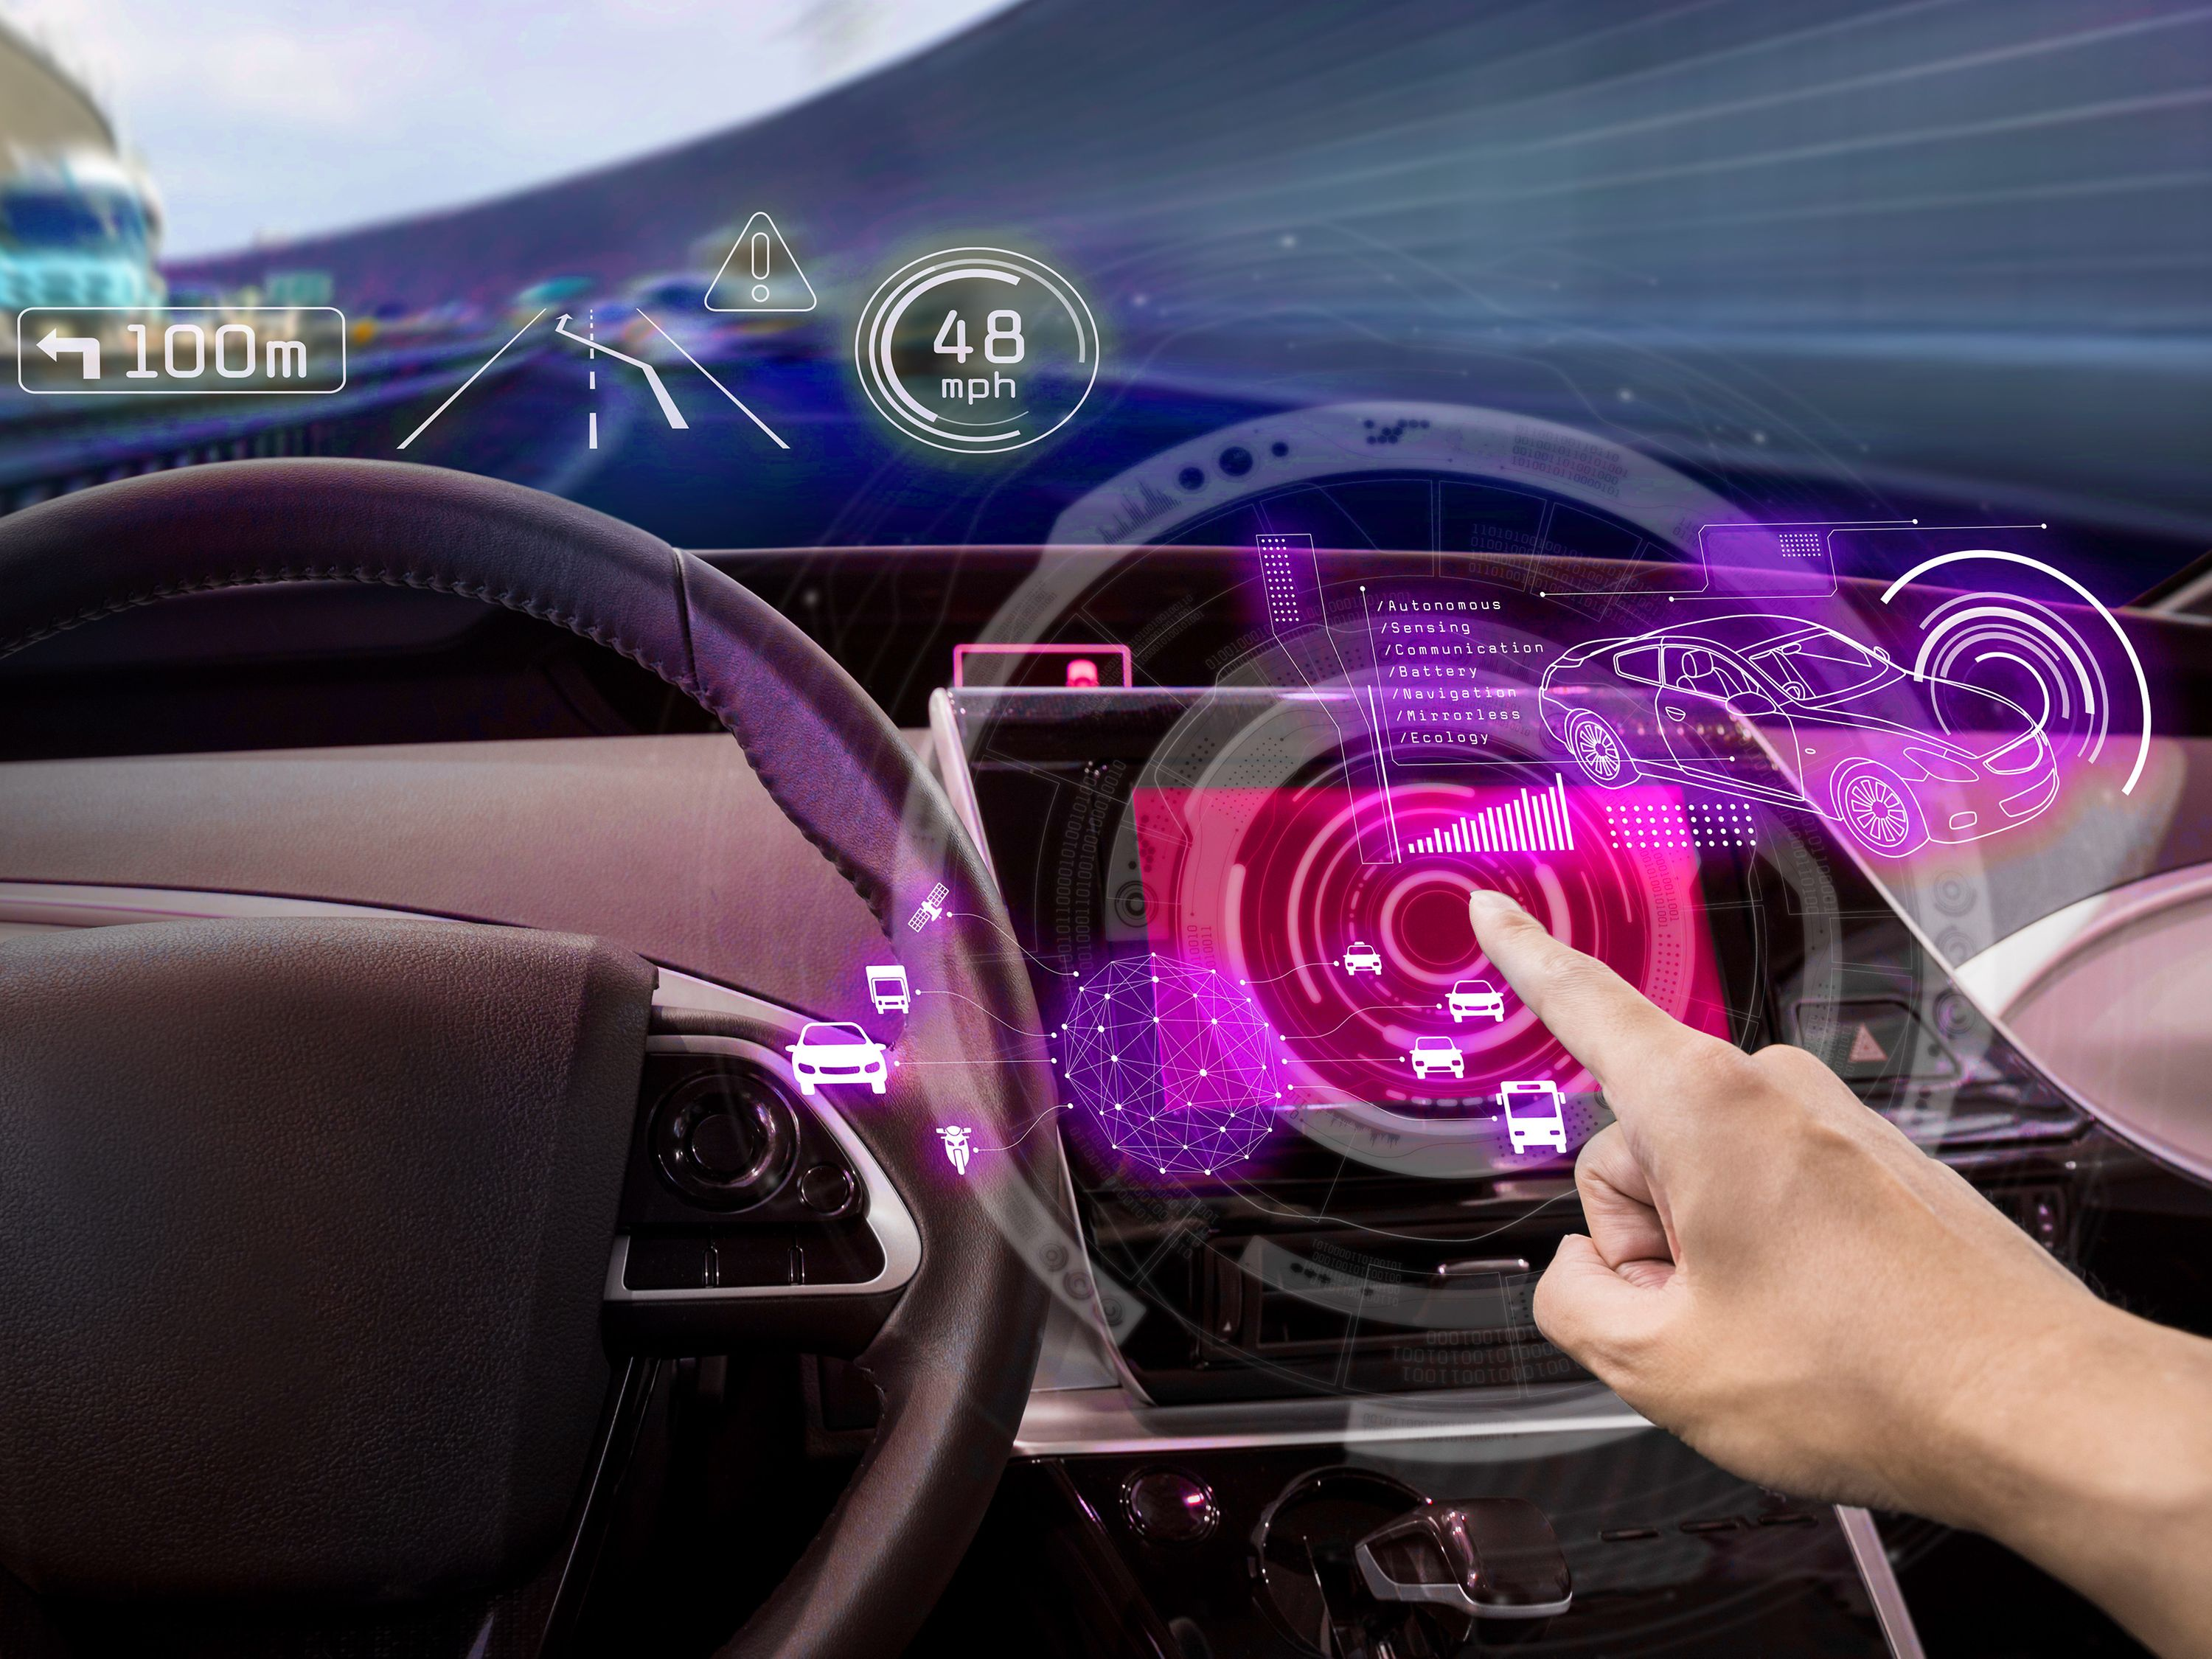
\includegraphics[width=0.47\textwidth]{figs/connected-vehicles.jpg}}\hfill
	~
	\subfloat[Augmented reality TODO: replace figure\label{fig:augmented-reality}]{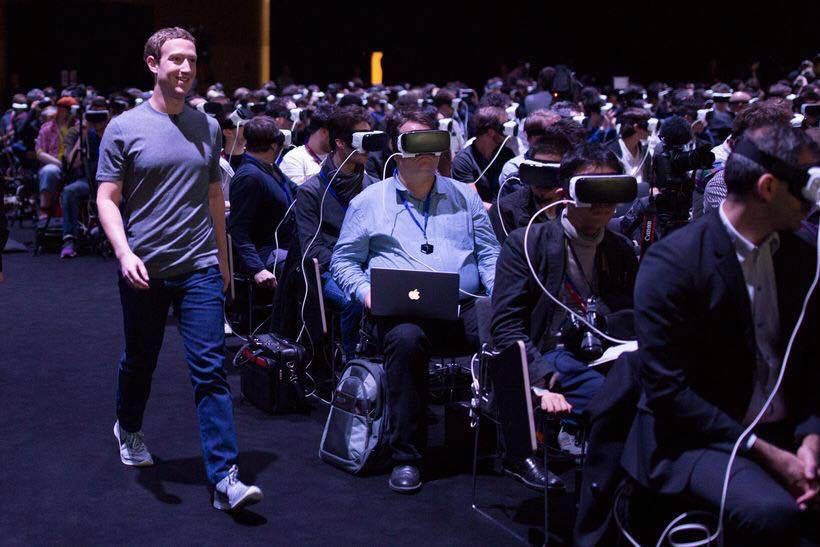
\includegraphics[width=0.53\textwidth]{figs/augmented-reality.jpg}}\hfill
	\caption{Different application can be enabled or benefit from the low-latency of services deployed to nearby edge servers} \label{fig:motivational-cases}
\end{figure}

\subsection{Low-Latency Applications}

The main motivation for shifting computation from cloud to the network edge is to mitigate latency~\cite{Bonomi2014}. In specific, real-time applications are the main candidates for benefiting of services deployed at nearby edge infrastructure. Among these, some have a higher degree of criticality with respect to latency and readiness of services (e.g., delay can have severe consequences to the users and/or the environment), whereas others can greatly benefit from lower latencies (e.g., by improving the user experience).

As an example of a critical application, connected vehicles (CV)~\cite{Bonomi:2012} are expected to be the computing device of the next decade, with each vehicle generating 25GB/hour of data~\cite{HitachiInternetOnWheels16}. In addition to local data analysis, more complex analysis shall be delegated to remote servers, which must respond quickly if the result involves critical information, e.g., the notification of an accident in the current path of the vehicle. With edge computing, computational resources located at mobile base stations or even composing the traffic infrastructure (e.g., highways) could provide low-latency services for connected vehicles passing by their coverage area.

Moreover, Augmented Reality (AR) is a type of application that would benefit from the low-latency of edge services~\cite{hu2015mobile,GarrigaMendonca2017}. These applications enrich the interaction of users with the physical
world by augmenting their vision of the reality with relevant information (e.g., historical information about buildings and monuments), modifying it (e.g., by translating captured text in a different language), or by adding virtual elements that can mimic interactions with the real world (e.g., virtual objects or creatures
from a fantasy game), or helping users fulfill physical tasks (e.g., by highlighting a free parking spot).

AR applications commonly depend on two key tasks: 1) extracting features from physical elements in the captured scene; and 2) matching these features against a feature database to obtain the corresponding information to be added to the scene. 

With the advent of mobile computing, AR applications can be deployed to companion devices like smartphones, tablets, and special purpose glasses. In many cases, these applications must process large volumes of data. Plus, this data can be volatile, which further limits the feasibility of storing it locally. Instead, data must be acquired from remote services. In order to augment the reality captured live from devices camera, the AR application needs to perform its tasks in a timely fashion, which poses a strong restriction on the latency requirement for remote services consumed. As such, a cloud-based solution tends to fail to meet this requirement~\cite{GarrigaMendonca2017}. 

%Additionally, image processing may over stress devices resources. This problem could be mitigated  
%architectural decision of where these tasks should be computed.

%AR applications that capture a live representation of the physical world, this reality must be augmented at real-time, meaning data must be retrieved in a timely fashion. Due to network latency, a cloud-based solution tends to fail. Accordingly, feature extraction task should be deployed near to client devices, e.g.., to edge servers. 

\begin{figure}[tbp]
	\centering
	\subfloat[Services are deployed to edge servers in order to reduce latency imposed by network communication with cloud servers \label{fig:cloud-to-edge}]{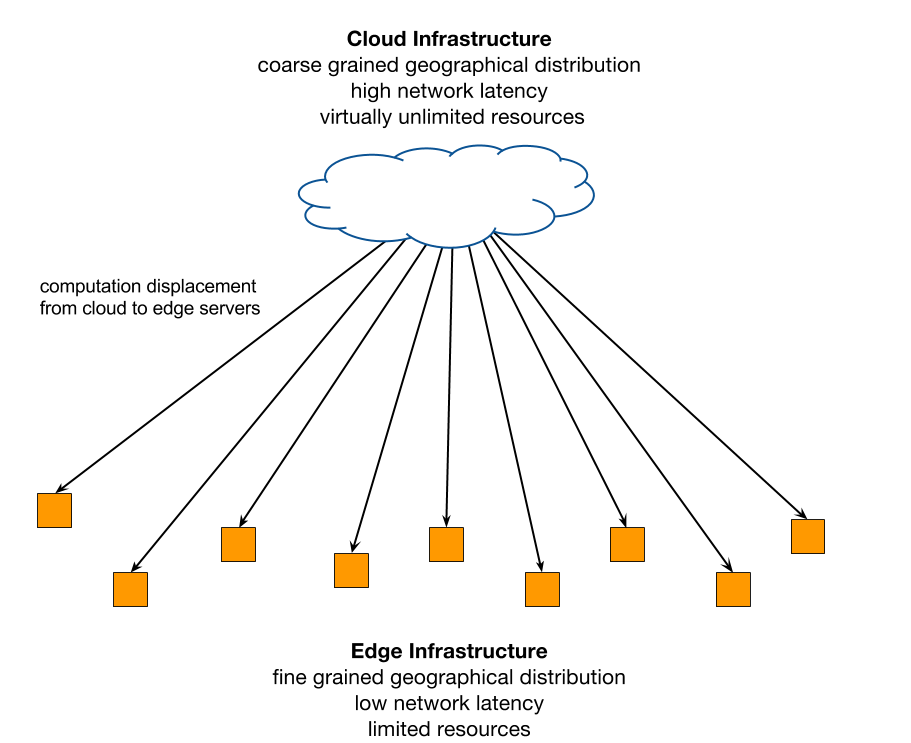
\includegraphics[width=0.45\textwidth,valign=t]{figs/cloud-to-edge.png}}\hfill
	~
	\subfloat[second caption.\label{fig:mobile-to-edge}] {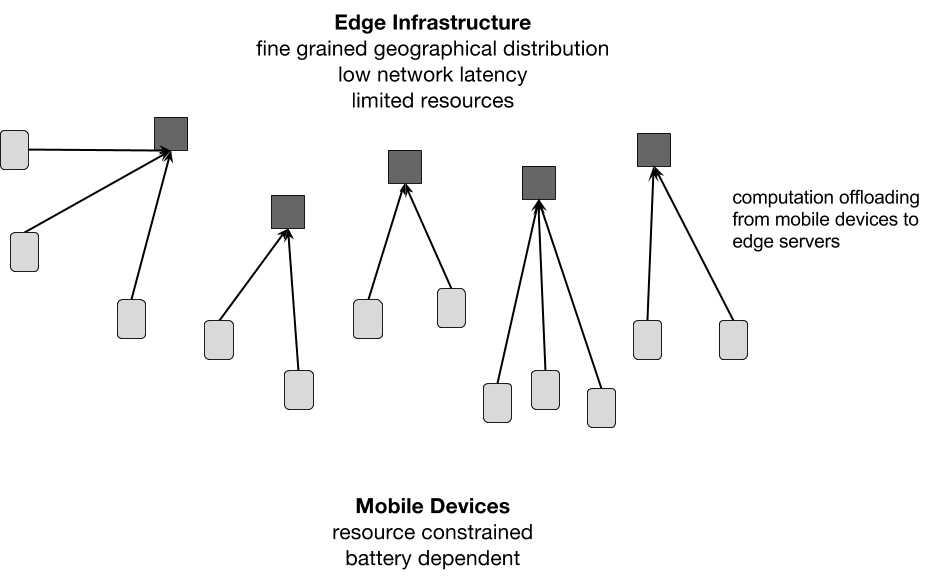
\includegraphics[width=0.55\textwidth,valign=t]{figs/mobile-to-edge.png}}\hfill
	\caption{General caption.} \label{fig:1}
\end{figure}

\subsection{Mobile Computation Offloading}

In addition to the problem of network latency, mobile devices exhibit limitations that may further motivate the use of edge computing as part of a continuum. 

For instance, some mobile applications rely on heavyweight tasks that can overstress the platform and limit the concurrent execution of other applications. Moreover, battery is a valuable resource that may be significantly affected by the kind of task performed by mobile devices. 

In the paradigm of Mobile Cloud Computing (MCC)~\cite{Khan:14}, this problem has been addressed with the offloading of mobile computation to cloud servers. This approach, however, is limited by network latency. In contrast, edge computing could be an alternative to allow heavyweight or complex computation with low-latency requirements to be offloaded from resource constrained devices to nearby servers.

%The paradigm of edge computing can be explored to mitigate the problems related to the resource limitations of mobile devices. For this, heavyweight computation from mobile applications could be offloaded to nearby edge servers. 

As an example, the previously mentioned feature extraction task from AR applications is a type of heavyweight computation based on image processing. Instead of performing it locally (as proposed in~\cite{Huang2012}), mobile devices could also offload this heavyweight task to nearby edge servers. 

\subsection{Computational Continuum}


\begin{figure}[tbp]
	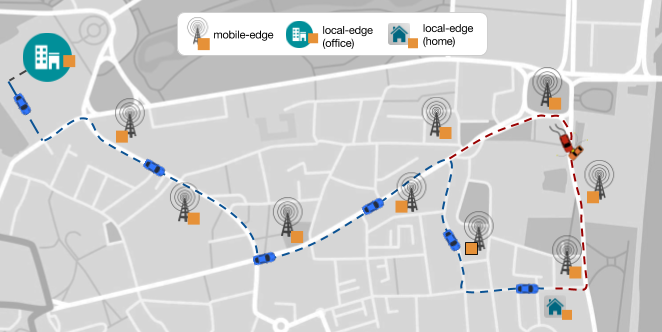
\includegraphics[width=0.9\textwidth]{figs/continuum.png}
	\caption{Heterogeneous applications (AR and CV) interact with services deployed along the computational continuum (cloud, mobile-edge, local-edge, and mobile)}
	\label{fig:continuum}
\end{figure}

Together, the computational resources from mobile, edge, and cloud computing have the potential of forming a \textit{continuum} on which new and disruptive types of applications can rely. Sometimes referred to as the Cloud-to-Things continuum, it enables the seamless convergence of infrastructure stretching from the cloud datacenter to devices on the network edge (including intermediate devices like ISP gateways, cellular base stations, and private cloud deployments) into a continuum of resources, to be provisioned to multiple tenants for hosting applications. Components of an application are hence able to run in a geo-distributed fashion using the services provided by the distributed infrastructure~\cite{GuptaIfogSim17}.   The key notion to bridge the gap in such a continuum is that of Edge\footnote{In the literature the term ``edge'' is often used interchangeably with the term ``fog''.} computing, whose defining characteristics are edge location, dense geographical distribution, large-scale of deployment, support for mobility, resource and interface heterogeneity, and interplay with the cloud properties in order to address requirements of mobile applications that need low latency with a wide and dense geographical distribution~\cite{Bonomi2014}.  

To illustrate such scenario, we put together the two case examples previously described as part of a continuum that starts in the user's office and finishes in his home (Fig.~\ref{fig:continuum}). 

First, let us assume the existence of a local edge server in the user's office (hereafter called \textit{local-edge}). This server is owned by the company to allow employees to extend the computational capabilities of mobile devices. In our example, the user makes use of a \textit{smartglass} application to craft three dimensional virtual objects added to his desk table.

After work, our user leaves his office and enters his CV. During its way home, the autonomous vehicle will make use of edge services deployed at servers located at cellular base stations and owned by telecoms (hereafter called \textit{mobile-edge}). The connected vehicle gets low-latency updates about the best plan to reach its destination. For example, within milliseconds, the vehicle is suggested to make a turn just in time to avoid the traffic formed by an accident a few blocks ahead. In particular, the new path consists of residential streets without coverage of mobile-edge services. The CV continue to fetch updates, this time from cloud services; the additional network latency is compensated with the low speed limit of the residential area.

Already at home, the user's smartphone gets in reach of communication with the local-edge server owned by him. In that day, the user finds out about a new mobile game application that makes use of AR. Upon installation, the local-edge server becomes aware of a new edge-compliant application and, meanwhile the game is already running locally, proceeds with the acquisition and deployment of the game services into the local-edge server. Once available, the client application becomes aware of these services and switches from local to edge with the purpose of preserving the smartphone's resources. Not only the game performance improves, but also the battery consumption is reduced.  

In the scenario described above, different parts of the continuum have been employed by user's devices. Whilst edge services were privileged, cloud services remain fundamental, as edge infrastructure was not always available. The services consumed by AR in a office scenario and the services consumed by a CV were pre-allocated. In contrast, a client application was able to make use of local resources from a mobile device until edge services were opportunistically made available. 

%services for which network latency is not disruptive are in the cloud (e.g., persistence, stateful components, and large part of the business logic). 

\section{Background}\label{sec:background}

\subsection{Cloud Computing and Virtualization}

The Cloud infrastructure is typically offered through different virtualization techniques and degrees. It is considered to be a black box: this means that we do not have access to the hypervisor or to
the underlying physical machines. A Cloud instance or \textit{node} is traditionally materialized as a Virtual Machine (VM). However,
nowadays a node might also be a container. Containers provide yet another virtualization technique that operates at the Operating System (OS) level, to create isolated views of the operating environment for different applications. A container has its own process space, virtualized network interface, and file system; and the operating system can allocate different amounts of resources (e.g., CPU, memory, and I/O) to each of them.

Multiple VMs are managed by a single hypervisor that resides on a single host operating system. Each VM then contains its own guest operating system, its own platform stack composed of different libraries, middleware, and application servers, and its own application code. On the other hand, containers are executed directly on top of the host operating system, optionally with the help
of a container manager like Docker\footnote{Docker -- \url{http://docker.com}}. Each container has its own platform stack and its own application code. Containers have various advantages when compared to VMs: they are more lightweight and they are faster to boot and
to terminate because they do not have to deal with a guest
operating system~\cite{FelterContainerVm15,SoletzContainerVirt14}.
%Industry is widely adopting containers as a means to favor portability and they are considered to be one of the main technological enablers of the DevOps movement [36]. Different development teams may use different operating systems and different platform stacks, making feature integration hard. However, thanks to containerization technology, features can be developed in isolation, with the guarantee that they will work the exact same way on any machine that supports containers.


\subsection{Serverless Computing and Functions as a Service}

Serverless Computing is an emerging and compelling paradigm for the deployment of cloud applications, largely due to the recent shift of enterprise application architectures to containers and microservices~\cite{baldini2017serverless}.  A Serverless Architecture is a refined cloud computing model to process requested functionality without pre-allocating any computing capability. Provider-managed containers are used to execute functions (often called lambdas), which are automatically provisioned on demand in few milliseconds, elastically scaled as needed, and ephemeral (may only last for one invocation)~\cite{Roberts:2016}. This approach allows one to write and deploy code without considering the server runtime
environment, resource allocation, load balancing, and scalability; all these aspects are automatically handled by the provider --- hence the term serverless. Functions are charged per invocation and per product of period of time and resource usage (with a millisecond granularity), leading to an almost perfect pay-as-you-go utility pricing model~\cite{MateosFaaster17}.  This allows companies to drastically reduce the cost of their infrastructures with regard to a typical monolithic architecture or even a microservices architecture~\cite{Villamizar2017lambda}.

The Serverless architecture has many benefits with respect to more traditional, server-based approaches. Functions share the runtime environment (typically a pool of containers), and the code specific to a particular application is small and stateless by design. Hence, the deployment of a pool of shared containers (workers) on a machine (or a cluster of machines) and the execution of some code onto any of them becomes inexpensive and efficient. In this manner, the serverless model represents the logical conclusion of the evolution of sharing between applications, from hardware to operating systems to (finally) the runtime environments themselves (Figure~\ref{fig:Evolution-of-Sharing}).

\begin{figure}
  \centering
    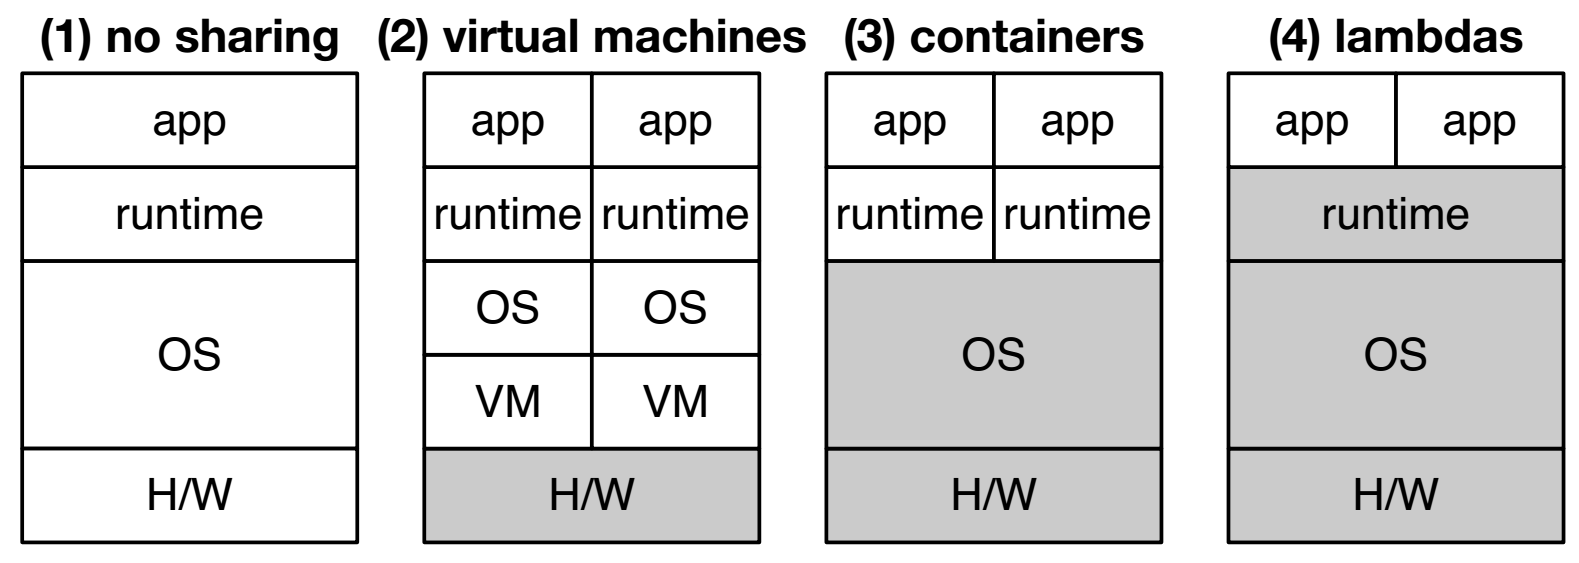
\includegraphics[width=0.7\textwidth]{figs/evolution-platform-sharing.png}    
    \caption{Evolution of platform sharing~\cite{Hendrickson:2016}}
    \label{fig:Evolution-of-Sharing}
\end{figure}


From the everything-as-a-service (XaaS) cloud computing taxonomies point of view, serverless is also known as Function-as-a-Service (FaaS)~\cite{MateosFaaster17}. There is still a controversy regarding how this differs from the Platform-as-a-Service (PaaS) model, which also abstracts away the management of servers. However, a Serverless model is a refinement of the platform layer where, unlike PaaS, developers can write arbitrary code and are not limited to using a pre-packaged application, but explicitly use functions as the deployment unit. 


From the automation point of view, it is important to consider the varying levels of control that the application developer has over the cloud infrastructure, as illustrated in Figure~\ref{fig:developer-control-serverless}. The Infrastructure-as-a-Service (IaaS) model is where less automation is achieved, while the application developer has the most control over both the application code and operating infrastructure. On the opposite extreme are the PaaS and SaaS models, where the developer is unaware of any infrastructure and uses pre-packaged applications and services. Consequently, she no longer has control since the infrastructure provision is completely automated. In the middle, where serverless lives, the application developer has control over the code they deploy into the Cloud, though that code has to be written in the form of stateless functions.  The operational aspects of deployment and maintenance are completely automated, fault-tolerant and
auto-scaling. In particular, the code may be scaled to zero where no servers are actually running when the user's function code is not used, and there is no cost to the user. This is in contrast to PaaS solutions where the user is often charged even during idle periods~\cite{baldini2017serverless}.

\begin{figure}[tbp]
	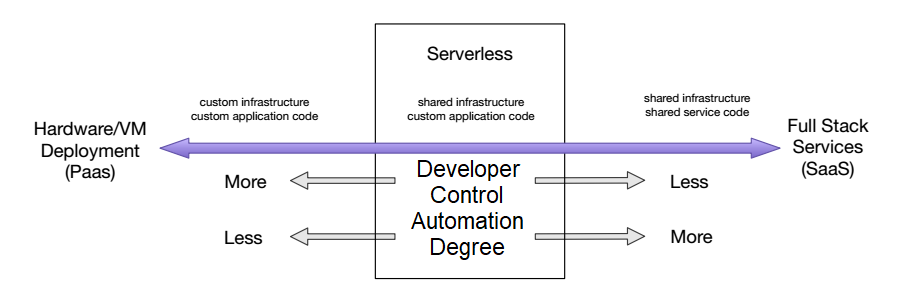
\includegraphics[width=0.9\textwidth]{figs/DeveloperControl.png}
	\caption{Automation degree in the XaaS taxonomy and the situation of serverless computing (adapted from~\cite{baldini2017serverless})}
	\label{fig:developer-control-serverless}
\end{figure}


Finally, from the Cloud providers point of view, serverless represents another revenue opportunity: the provider offers an ecosystem of preexisting services that augment the user's functions. For example, there may be services to manage state, record and monitor logs, send alerts, trigger events, or perform authentication and authorization. Such rich ecosystems can be attractive to developers, leading to an increased adoption of the vendor's solutions. Several cloud providers have developed serverless platforms recently, many of which are still in their explicit or implicit beta testing phase\footnote{\url{https://blog.zhaw.ch/icclab/faas-function-hosting-services-and-their-technical-characteristics}}. Table~\ref{tab:FaaS-providers-and} summarizes the main serverless solutions, with AWS Lambda that appeared 1.5 years before the others (around 2015). All these alternatives provide similar capabilities, while IBM/Apache Openwhisk is the only open-source solution among the major vendors. Other academic alternatives exist, such as OpenLambda\cite{Hendrickson:2016}, but these are mostly suitable for research purposes.

\begin{table}[hbt]
\centering
\caption{Serverless providers and supported languages\label{tab:FaaS-providers-and}}{
\begin{tabular}{ll}
\toprule 
\textbf{Provider} & \textbf{Languages}\tabularnewline
\midrule
AWS Lambda & Node.js, Java, Python\tabularnewline
Google Cloud Functions & Node.js\tabularnewline
Azure Functions & Node.js, C\#\tabularnewline
IBM OpenWhisk & Node.js, Swift, Binary (Docker)\tabularnewline
Webtask.io & Node.js\tabularnewline
OpenLambda & Python\tabularnewline
\bottomrule
\end{tabular}}
\end{table}

%provide what is been called as \textit{Functions as a Service} (FaaS). A FaaS is a realization of the serverless paradigm in which stateless functions  


\subsection{Edge Computing}

Edge computing can be defined by the set of technologies that enable computation to be performed at the network edge~\cite{Shi:2016}. Its main goal is to allow data produced and consumed at the network edge to be processed with low-latency and without overstressing the more centralized cloud infrastructure.

As examples of edge technologies, Cloudlets~\cite{Satyanarayanan:2009} have been first presented as mobile cloud servers that can be positioned at strategic locations to provide computing resources to resource constrained devices with low-latency. 
%with expected high density of users (e.g., at concert halls, stadiums) or areas with temporary infrastructure limitations (e.g., after disasters). 
Additionally, mobile edge computing (MEC)~\cite{ahmed2016isco} relies on cellular infrastructure to enable a low-latency communication between user equipment (i.e., mobile devices) and servers. 

The main motivation for shifting computation from cloud to the network edge is the mitigation of network latency~\cite{Bonomi2014}. In specific, real-time applications are the main candidates for benefiting of services deployed at nearby edge infrastructure. For example, Augmented Reality (AR) is a type of application that would benefit from the low-latency of edge services~\cite{hu2015mobile,GarrigaMendonca2017}. Moreover, mobile devices exhibit limitations that may further motivate the use of edge computing as part of a continuum: some mobile applications rely on heavyweight tasks that can overstress the platform and limit the concurrent execution of other applications; and the battery is a valuable resource that may be significantly affected by the kind of task performed locally~\cite{Carroll:2010}. 

%In addition to the aforementioned types of edge computing, in this paper we explore the usage of \textit{local-edge} as servers deployed as part of a building infrastructure to further improve the computational power of nearby devices. 
\section{A3-E}\label{sec:A3-E}

%\begin{figure}[tbp]
%	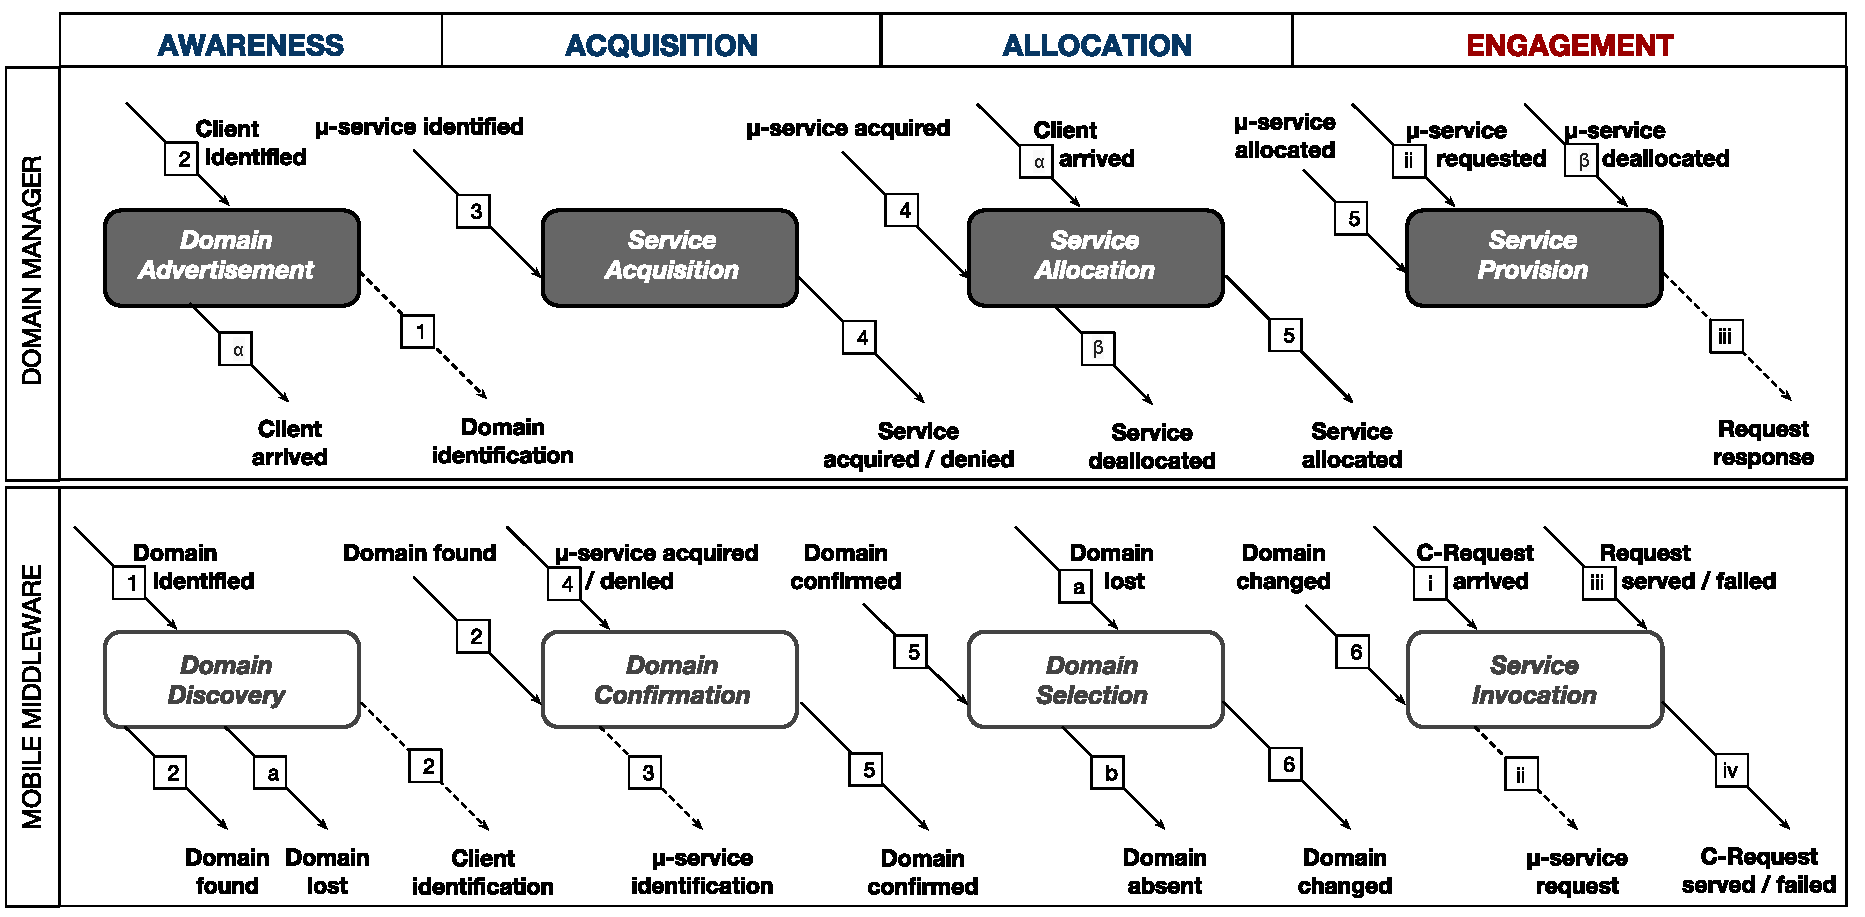
\includegraphics[width=0.92\textwidth]{figs/A3-E-process}
%%	\setlength{\belowcaptionskip}{-10pt}
%	\caption{A3-E overview. A3-E's activities are carried out by a \textit{domain manager} and a \textit{mobile middleware}, and coordinate through incoming ($\rightarrow$) and outgoing ($\leftarrow$) asynchronous events.}
%	\label{fig:A3-E-process}
%\end{figure}

\begin{figure}[tbp]
	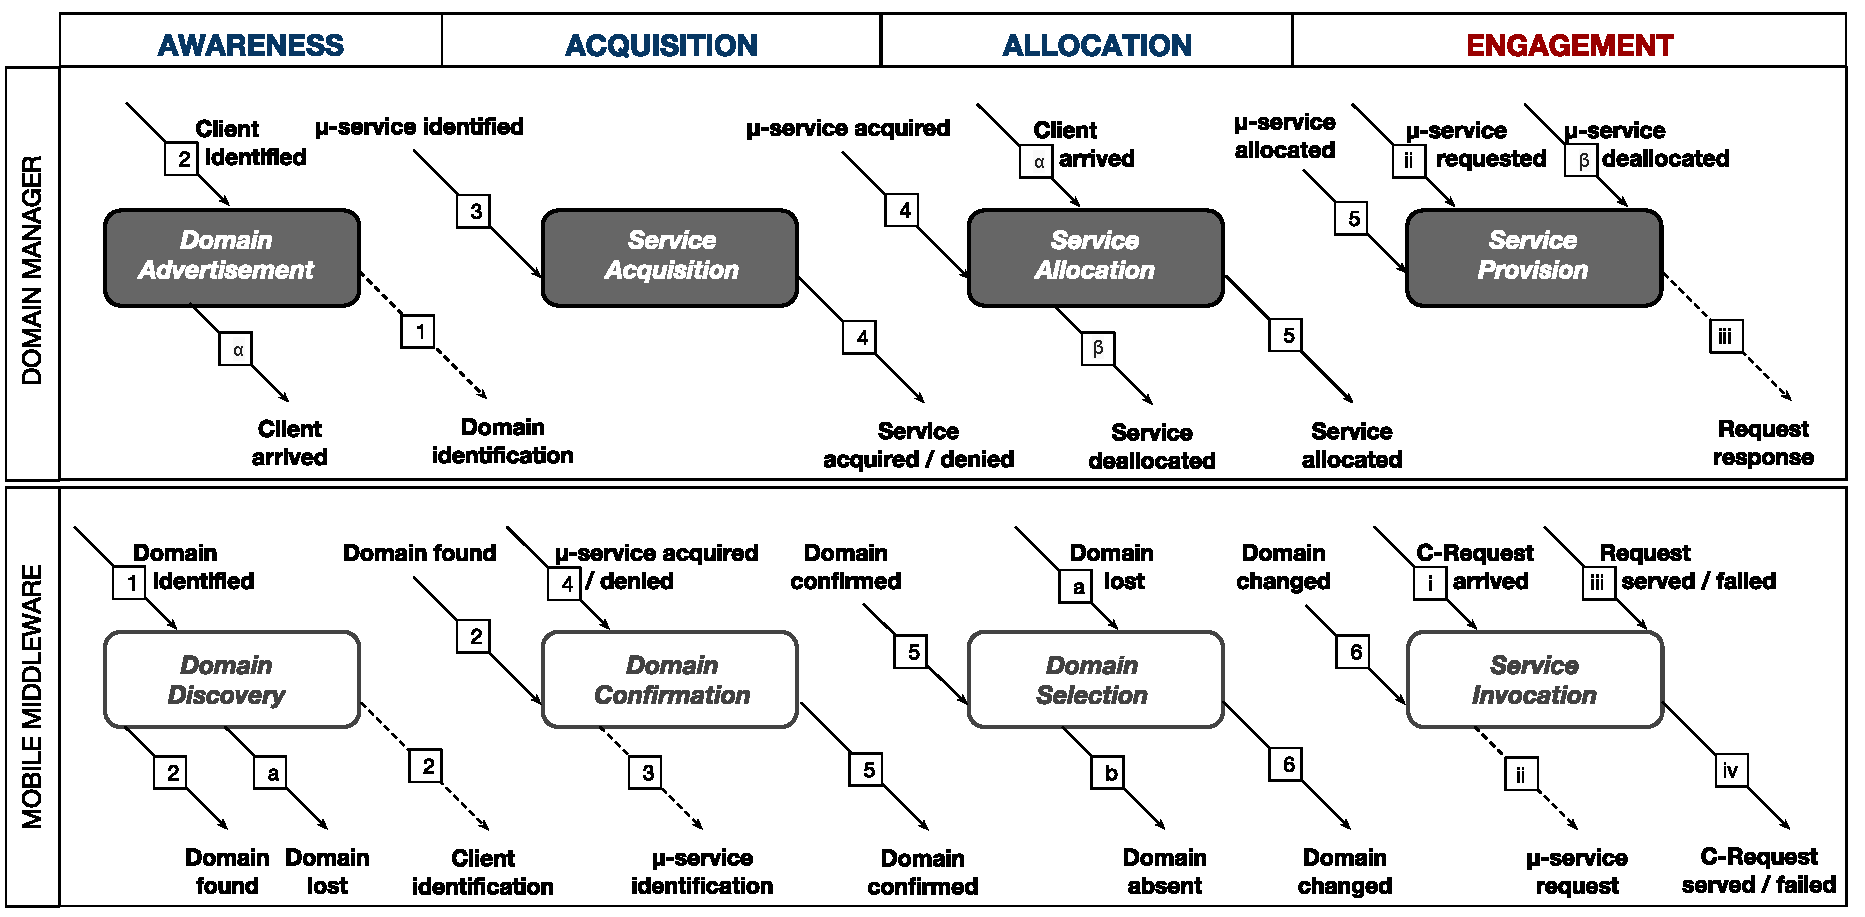
\includegraphics[width=0.85\textwidth]{figs/A3-E-process}
	%	\setlength{\belowcaptionskip}{-10pt}
	\caption{A3-E overview. A3-E's activities --- (AW)areness, (AQ)uisition, (AL)location, (E)ngagement --- are carried out by a \textit{domain manager} and a \textit{mobile middleware}, and coordinate through asynchronous events depicted by and identified as follows: \textit{domain identification}~(DI), \textit{client identification}~(CI), \textit{client arrived}~(CA),\textit{client left}~(CL),\textit{$\mu$-service identified}~($\mu$I), \textit{$\mu$-service acquired}~($\mu$AQ), \textit{$\mu$-service allocated}~($\mu$AL), \textit{$\mu$-service (deallocated}~($\mu$DA), \textit{domain found}~(DF), \textit{domain lost}~(DL), \textit{domain ready}~(DR), \textit{domain changed}~(DS), \textit{execution time}~($\Delta$EX), \textit{$\mu$-service request}~($\mu$RQ), \textit{$\mu$-service response}~($\mu$RS), \textit{C-Request}~(C-RQ).}
	\label{fig:A3-E-process}
\end{figure}

%First and foremost, A3-E's main objective is to enable the efficient and scalable placement of $\mu$-services along the continuum. In A3-E, clients and providers autonomously interact and decide for the placement of services according to the context. Moreover,  

To realize the mobile-edge-cloud continuum, we propose A3-E, a model supporting the self-management of continuum $\mu$-service life-cycles. A3-E inherits its name from its four main activities -- namely, \textit{(\textbf{A})wareness, (\textbf{A})cquisition, (\textbf{A})llocation, and (\textbf{E})ngagement}. 

A3-E targets 
the efficient and scalable placement of $\mu$-services along the continuum and the satisfaction of application requirements such as maximum service latency, battery consumption, and availability. 
To achieve it, clients and heterogeneous domains take part in the automated and opportunistic decision of which continuum resources --- among those of mobile, edge, and cloud --- should be employed in provisioning each of the $\mu$-service required by continuum applications. 

%A3-E targets 
%%the materialization of the continuum by means of an
%the efficient and scalable placement of $\mu$-services along the continuum. 
%To achieve it, clients and heterogeneous \textit{mobile, edge, and cloud} domains take part in the \textit{automated} and \textit{decentralized} decision of which continuum resources should be employed in provisioning each of the $\mu$-services required by continuum applications.% according to the context of operation.


%A3-E exploits the FaaS paradigm and propose additional mechanisms for 

Figure~\ref{fig:A3-E-process} illustrates each activity in A3-E. 
Activities are refined by procedures that coordinate through asynchronous events and are carried out by a \textit{domain manager} and by a \textit{mobile middleware}. 
%Activities from both sides are coordinated through signals and events. 
To address the intrinsic heterogeneity of the continuum, A3-E is flexible with respect to how each of its activities is actually implemented. 
%For each phase, the main activities of a \textit{domain} and a \textit{client} are depicted along with their mutual relative state at the moment the phase starts: for a domain, a service state ranges from \textit{Free} to \textit{Allocated}, whilst a domain state ranges from \textit{Away} to \textit{Selected} for a client. 
%More precisely, Fig.~\ref{fig:A3-E-process} refers to the activities and states (in parenthesis) of a single client-domain interaction.

%Next, we detail each main activity in A3-E, starting from the most general one, i.e., the one that applies to all types of client-domain interaction, and moving towards the more specific ones.


%\subsection{A3-E Process: Phases}\label{sec:A3-E-process}

%Next, the four A3-E phases are further described and mapped to the requirements elicited in  Section~\ref{sec:requirements}. Later on, other possible instances of the A3-E model are correlated with scenarios of the compute continuum.


\subsection{Awareness}\label{sec:A3-E-awareness}

%From the provider's viewpoint, the main purpose of Awareness is to enable domains to opportunistically and pro-actively initialize the Acquisition and Allocation activities. %, based on the awareness of devices in a domain's coverage area. 
%In turn, clients benefit from Awareness with the dynamic discovery and profiling of domains that can provide the $\mu$-services they need.

%A3-E's Awareness models (i) the discovery of domains and (ii) the discovery of continuum applications in one of its domains' area of coverage, indicating the imminent need for specific $\mu$-services. 




The latency of continuum $\mu$-services can be decomposed into three parts: \textit{acquisition delay} ($\Delta AQ$), \textit{allocation delay} ($\Delta AL$), and \textit{execution delay} ($\Delta E$). FaaS platforms like AWS Lambda~\cite{AWSLambda}
%~\footnote{https://docs.aws.amazon.com/lambda/latest/dg/running-lambda-code.html}
and OpenWhisk~\cite{OpenWhisk} adopt a \textit{cold start} policy in which $\mu$-services are allocated after their first call following a period of idleness. This latency, however, may be disruptive for some applications. 
%To satisfy the maximum accepted latency of provided $\mu$-services, a \textit{domain manager} mitigates each component as follows: 

%In comparison, %the proposed mutual client-provider awareness 
A3-E's Awareness has two benefits: (i) it alleviates $\Delta AL$ (cold starts) by pro-actively allocating $\mu$-services just before they are needed; and (ii) it reduces $\Delta AQ$ and enables $\mu$-service acquisition to be opportunistic (i.e., on demand) by triggering the download and installation of new $\mu$-services as soon as the client becomes active in a specific domain (e.g., by starting the application or by entering an edge domain's area).

%TODO [Danilo] this kind of detail fits better in the implementation, doesn't it?
While cloud domains are not likely to change, and may be set-up statically by clients,% to realize this activity
edge domains must advertise their existence (\textit{domain identification}) using protocols that are compatible with its network infrastructure: for instance, through IP broadcasting in local-edge, and through Evolved Multimedia Broadcast/Multicast Service (eMBMS) in mobile-edge~\cite{lecompte2012evolved,etsimec16:03}. 
In particular, edge domains exploit locality by triggering a \textit{client left} event once mobile devices leave its coverage area, whilst cloud domains rely on adjustable \textit{timeout}.% for triggering this event.




%Throughout Awareness, the domain manager handles the following event:

%{\small
%\begin{itemize}
%	
%	\item \textbf{Client identified:} triggered when a new client enters the domain's coverage area. The manager must react with the triggering of a \textit{client arrived} and \textit{$\mu$-service identified} events for each $\mu$-service required by the client.
%	
%\end{itemize}
%}%

From the client's perspective, Awareness corresponds to the discovery of domains (source of \textit{domain found} and \textit{domain lost} events) and the advertisement of required $\mu$-services through a \textit{client identification} signal containing their metadata (name, repository url), upon which the domain manager triggers both \textit{client arrived} and \textit{$\mu$-service identified} events.% for each required $\mu$-service. 

To realize this activity, special purpose HTTP endpoints can be used for cloud domains; protocols from local area networks (e.g., UDP, IP multicast) are used for local-edge domains; eMBMS protocols (e.g., FLUTE~\cite{lecompte2012evolved}) which are carried over traditional UDP and IP multicast toward end-user devices, are used for mobile-edge domains; and system-level signals (e.g., broadcast intents in Android platforms) are used by mobile domains.

%[Danilo] 2ndR: this paragraph is poor
%In our running example, the mobile-edge and local-edge domains must advertise their existence to our user's device, which in turn identifies the AR and Image Editing applications. The same holds for the hotel's local-edge domain and the MG application. %In all cases, cloud and edge domains can employ Awareness to opportunistically fetch, install, and allocate instances of required $\mu$-services.


%The mobile middleware, in turn, realizes Awareness with the discovery of cloud and edge domains. In particular, 
%During Awareness, the mobile middleware handles the following event:
%
%{\small
%\begin{itemize}
%	
%	\item \textbf{Domain identified:} triggered when a domain is found. The middleware must react with the triggering of a \textit{domain found} event and a \textit{client identification} signal to the domain manager.
%	
%\end{itemize}
%}%

%To implement Awareness, 

%It copes with the need for efficiency and scalability of finely distributed edge domains by allowing acquisition and/or allocation of services to happen just in time, i.e., just before the client application needs them.
%and enables not only functions to be allocated, but also acquired in an opportunistic fashion.
%The benefit lies in the anticipation of (opportunistic) services setup with respect to the arrival of the first service request, i.e., in the mitigation of service setup delay (also known as cold start). Since cloud domains cover a large area, the later do not employ the awareness phase. Needless to say, mobile domains do not require awareness for sharing the same platform with client applications.

%TODO [Danilo] Commented-out in favor of a more abstract description in terms of events, as broadcasting is something local-edge specific
%The DSM achieves this by broadcasting its existence and by waiting for clients to pass along their requirements. In our running example this occurs when the user's domestic local-edge server becomes aware of the new mobile game that the user had just installed. 
%%nd the discovery of client applications along with their requirements (i.e., services). The later are passed to the following phase of acquisition.
%%then receive all client application requirements (i.e., services) as soon as the client's mobile device enters the domain's coverage area, and then pro-actively starting acquisition and allocation. 
%%For example, in the real-time translation application previously introduced, the service setup delay was mitigated by having the acquisition of the data and codebase composing the service to start as soon as the user entered the edge domain's coverage area.
%%For example, the setup of services required by the mobile multiplayer game application by the user's local-edge server follows the awareness of a new application.
%From the client's perspective, the awareness phase models the discovery of domains, and corresponding $\mu$-services, whose network addresses are not previously known. In particular, it tackles edge domains that are integrated with the local network infrastructures of buildings and public spaces. This modality contrasts with cloud which are accessed through DNS and traffic managers. Needless to say, the awareness phase is not considered by mobile domains. The CSM intercepts the provider's broadcast messages, and reacts by sending back its application requirements. This process should happen once, and in a timely fashion, upon connection to new networks to mitigate battery consumption. As an example, the local-edge server in our user's home is discovered when her mobile device connects to her domestic Wi-Fi network. 


%Once the domain is ready, this domain becomes an alternative for the provisioning of services required by the many applications (e.g., the mobile multiplayer game) hosted by the user's smartphone, tablet, and/or other of his IoT gadgets. 


%Finally, the Awareness phase has the following purposes: 1) to enable domains to pro-actively initialize the acquisition and allocation phases based on its awareness of applications whose hosting devices happens to be in the domain coverage area (Req.~\textbf{R2.3}); and 2) to enable clients to discover the address of local domains (Req.~\textbf{R2.2}).

%From the domains perspective, the awareness of clients presence in their coverage area allows a proactive download and installation of services artifacts (acquisition phase) and/or the allocation of services (allocation phase) potentially before a first request to that service arrives, alleviating the delay introduced by services setup.  From the clients perspective, the awareness phase increases the range of alternatives from the continuum that can be used to satisfy their requirements.

%Such behavior allows that are opportunistically acquired and/or allocated to mitigate their setup delay by triggering these phases upon awareness of client(s) in their coverage area.

%From the domain-side, the lack of awareness of clients in the domain coverage area prevents triggering the acquisition and subsequently allocation phases based on this event. From the client-side, the lack of awareness from surrounding domains prevents them to make the decision of which domains to use. In the later case, clients must rely on external components to reach servers (e.g., traffic managers and DNS servers).

\subsection{Acquisition}\label{sec:A3-E-acquisition}

A3-E's \textit{Acquisition} models the automated download and installation of continuum $\mu$-service artifacts, and the confirmation of the domain's capability in providing that $\mu$-service. Its ultimate goal is to mitigate the use of domain resources before the $\mu$-service is actually needed, while also facilitating IT operations (Ops) for developers and administrators. 

Ops mitigation is particularly important in (finely distributed) edge domains, since the manual administration of a large number of $\mu$-services can prove cumbersome and expensive. Nevertheless, this can also prove useful for cloud domains. Indeed, to the best of our knowledge, current FaaS platforms only support uploading (pushing) functions through public interfaces. 

Acquisition is autonomously managed, therefore it allows $\mu$-services to be downloaded 
%(e.g., pulled from a repository) 
and installed on demand. A domain manager fetches the artifacts (e.g., compiled classes and dependencies) from a repository upon the arrival of a \textit{$\mu$-service identified} event. Note that mobile domains are exempt of performing Acquisition as local $\mu$-services are assumed to be downloaded and installed along with the client application and the mobile middleware. 

% In addition to function sources, artifacts may comprise data and libraries needed by the service.

%Throughout Acquisition, the domain manager handles the following event:
%
%{\small
%\begin{itemize}
%	
%	\item \textbf{$\mu$-service identified:} indicates the request for deployment of a new $\mu$-service. The manager must proceed with the download and installation of the $\mu$-service, followed by the triggering of a \textit{service acquired} (or \textit{denied}) signal/event according to the activity outcome.
%	%its capability in providing that $\mu$-service.
%	
%	%\item \textbf{Client arrived:} triggered when a new client entered the domain's coverage area. The manager must react with 
%	
%\end{itemize}
%}%

%In this phase, the domain manager receives a set of application requirements from the client's CSM, namely the list of $\mu$-services and the URL of their repositories. The desired $\mu$-service artifacts are then downloaded and installed, at which point the DSM informs the client whether the $\mu$-services can be considered ``acquired'' or not. 
%Throughout the $\mu$-services' life-cycles, the DSM periodically checks for new versions of acquired services and updates them accordingly. 
%As an example, the services consumed by both AR applications introduced early can be autonomously acquired on demand by the local-edge servers in the user's office and home, preventing the company and the user to perform such operation. 
%In case the service has already been acquired or as the acquisition finishes, clients should add that domain to their list of available domains. 

From the client's perspective, Acquisition corresponds to the confirmation (or denial) of a domain's capability in providing the $\mu$-services required by the application. After a \textit{domain found} event, the mobile middleware listens for a \textit{$\mu$-service acquired} signal --- to be handled with the update of a list of capable domains and the subsequent triggering of a \textit{domain confirmed} (or \textit{denied}) event.

In our running example, the assets composing the $\mu$-services from the AR, Image Editing, and MG applications are once fetched and installed by the two local-edge domains upon arrival of a first \textit{$\mu$-service identified} event. While this is achieved, the applications momentarily continue to rely on their own mobile domain, or on any other domain on which $\mu$-services have already been acquired and allocated due to a previous client-domain interaction (e.g., the mobile-edge domains in our example skip Acquisition of AR artifacts due to previous contact with tourist devices).

%
%During this activity, the mobile middleware deals with the following events:
%
%{\small
%\begin{itemize}
%	
%	\item \textbf{Domain found:} indicates a potential domain for a $\mu$-service has been found. The middleware must proceed with the \textit{$\mu$-service identification} signal (if the domain is new) followed by the triggering of a \textit{domain confirmed} event.	
%	
%	\item \textbf{$\mu$-service acquired:} indicates a successful acquisition of a previously identified $\mu$-service. The middleware must react with the triggering of a \textit{domain confirmed} event.
%	
%	\item \textbf{$\mu$-service denied:} indicates the failure in acquiring and/or deploying a $\mu$-service. The middleware must proceed with the blacklisting of that domain. 
%	
%\end{itemize}
%}%


 %follow the identification of the domain's capability in providing the requested service. This phase is realized by the CSM with the following sub-process: the CSM should expect a confirmation from the DSM regarding its compliance in providing the service required by the application. Once confirmed, the CSM adds that domain to a list of available domains used by the client-side allocation phase. 

%As an example, a real-time translation application from/to streams of different spoken languages require services with low-latency. The translation can either rely on local services provided by the mobile domain (zero network latency) or on remote services provided by the edge domain (low network latency). Given the battery constraints of the mobile device, edge services are preferred. Instead of having all artifacts pre-installed, the edge's DSM acquires the data and codebase from a repository informed by the CSM upon detection of the user in its coverage area. The setup process takes no more than a minute, during which local services were consumed. Once the setup is ready, the application can start streaming captured conversations to edge-based services, which in turn reply with a translated audio stream.

%From the domain-side, the lack of acquisition implies that service assets must be previously made available. Nonetheless, the preliminary acquisition of a large number of assets is limited by the domain storage capability. 

%Conversely, the automated and opportunistic acquisition of service assets improves storage efficiency with the cost of a setup time $\Delta_{AQ}$. For instance, domains that become aware of clients' requirements may pro-actively start the acquisition phase and become ready for allocation before the first service request arrives.

%otherwise, domains must rely on the detection of a first service request or some other triggering condition to start the acquisition phase and, after setup time $\Delta_A$, become ready for allocation. 



\subsection{Allocation}\label{sec:A3-E-allocation}

%\begin{figure}[thbp]
%	\centering
%	\captionsetup[subfigure]{width=0.4\textwidth}	
%	\null\hfill
%	\subfloat[Domain $\mu$-services allocation control loop; domains must monitor the QoS of deployed $\mu$-services and adapt its allocation scheme to prevent SLA violations.\label{fig:service-allocation-loop}]{ 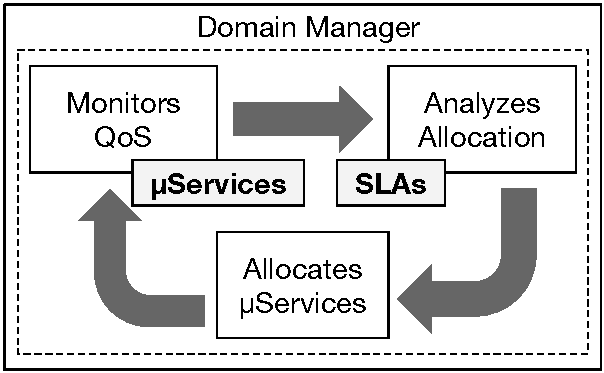
\includegraphics[width=0.4\textwidth]{figs/service-allocation-loop}}
%	\captionsetup[subfigure]{width=0.4\textwidth}	
%	\hfill
%	\subfloat[Per $\mu$-service domain selection control loop; clients monitor $\mu$-services from available domains and select the one that best satisfies its requirements.\label{fig:domain-selection-loop}] {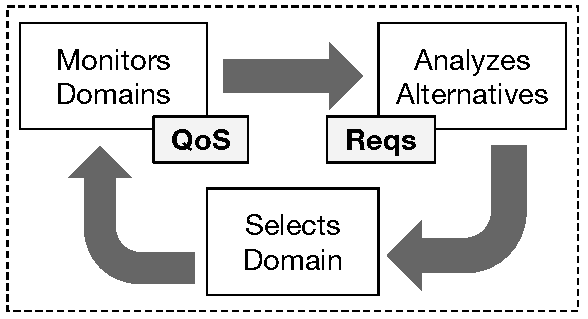
\includegraphics[width=0.4\textwidth]{figs/domain-selection-loop}}
%	\hfill\null
%	\caption{Self-management loops for domain-side $\mu$-services allocation and client-side domain selection}\label{fig:allocation-loops}
%\end{figure}


\textit{Allocation} models the deployment of continuum $\mu$-services on a pool of resources provided by the domain. It also captures the client-side selection of domains for each of the $\mu$-services employed by the application.

%From the domain's perspective, the allocation phase models the placement of $\mu$-services on the domain's resources, i.e., on its pool of servers, virtual machines, and containers. At the beginning of this phase, $\mu$-service artifacts have been \textit{acquired} by the domain, and the client has been \textit{notified} of this.

The scope of the provider-side Allocation is limited by its domain boundaries. Cloud domains allocate $\mu$-service instances to containers in resourceful datacenters covering a large area. On the other hand, edge domains rely on containers from one or more (virtual) machines serving an office or a building (local-edge) or a 5G base station area (mobile-edge). Finally, the allocation of $\mu$-services into mobile domain resources is platform specific (e.g., Android service life-cycle).

%pre-allocated and no allocation is needed.

%In this paper, we do not consider inter-domain cooperation (e.g., placement among different domains).

Existing FaaS platforms handle Allocation with on demand instantiation of containers after a first request, which may be kept \textit{warm} before being deallocated after a period of idleness~\cite{AWSLambda, OpenWhisk}. A3-E generalizes this mechanism as a self-management loop~\cite{kephart2003vision}
in which $\mu$-service instances are allocated to cloud and edge domain resources to guarantee that service latency and availability of each provided $\mu$-service are in-line with the desired SLA. 

%To better express this problem, let's consider the set of $\mu$-services $S = \{s_j \mid j = 0,1,...,J\}$.
%%In turn, $F_i = \{f_{i,j}\}_j$ defines the set of instances of $s_i$, with $0 \le j \le n_i$.
%%Instances for each $\mu$-service are defined by the set $F_i = \{f_{i,j}\}_j$, with $0 \le j \le n_i$.
%Vector $\bar{c} = (c_1, ..., c_J)$ holds the number of instances for all $\mu$-services. Each instance is bound to a container; resources allocated to each container 
%%Each $s_j \in S$ has a corresponding set of instances $F_j = \{f_{j,i} \mid i = 0,1,...,I_j\}$, where each instance is bound to a container. 
%(e.g., CPU and memory) are considered fixed and equal for all $\mu$-services, coherently to the architecture of FaaS frameworks such as OpenWhisk~\cite{OpenWhisk}.
%
%Now let's assume that each provided $\mu$-service $s_i \in S$ is bound to an SLA specifying its \textit{maximum accepted service latency} $\Delta_j$ 
%as well as the minimum/maximum number of service instances $Kmin_{j}/Kmax_{j}$. %, and a relative priority $p_i$. 
%Given the fluctuations in the workload and the response time $\tau_j$ (comprising both \textit{queue time} and \textit{service time}) of each $\mu$-service $s_j \in S$, the aim of a \textit{domain manager} is to find the minimum $c_j$ for each $\mu$-service so that, $\forall s_j \in S,\ \tau_j \le \Delta_j\ \wedge\ Kmin_j \le c_j \le Kmax_j$. 

To achieve this goal, the self-management \textit{monitor} ($M$ in Fig.~\ref{fig:A3-E-process}) calculates the \textit{arrival rate} ($\alpha_j$) and the \textit{response time} ($\tau_j$), as well as the \textit{number of clients} for each provided $\mu$-service ($s_{j} \in S$). The first two parameters are updated after each $\mu$-service execution ($QoS$ in Fig.~\ref{fig:A3-E-process}), whilst the second depends on \textit{client arrived} and \textit{client left} events from Awareness (respectively $CA$ and $CL$ in Fig.~\ref{fig:A3-E-process}). The \textit{analyzer} ($A$ in Fig.~\ref{fig:A3-E-process}) then outputs the number of instances $c_j$ for each $s_j \in S$ so that $\forall s_j \in S,\ \tau_j \le \Delta_j\ \wedge\ Kmin_j \le c_j \le Kmax_j$. It is up to the \textit{planner} ($P$ in Fig.~\ref{fig:A3-E-process}) to decide if and how to cope with the new allocation scheme based on the domain's resources (memory and CPU) and SLA for each $s_j \in S$.
%Moreover, the monitoring procedure considers the response time ($\tau_j$) and 
To mitigate \textit{cold start} ($\Delta 2_j$), the planner reacts to a \textit{client arrived} event by anticipating container allocation if resources are available at that loop iteration; and by keeping containers allocated (\textit{warm}) after a $\mu$-service execution. Finally, the \textit{executor} ($E$ in Fig.~\ref{fig:A3-E-process}) carries out the new allocation scheme by means of commands to the container platform (i.e., Docker).

%Throughout Allocation, the domain manager reacts to a 
%a \textit{$\mu$-service acquired} event --- indicating that the function(s) and dependencies have been fetched, and that the $\mu$-service is ready to be deployed ---  
%%The domain manager must react 
%by including this $\mu$-service in its self-management loop handling allocation. 
%%\textbf{THIS SELF-MANAGEMENT LOOP IS NOT WELL INTRODUCED. IT KIND OF DROPS OUT OF NOWHERE} 
%Also, to mitigate cold starts, the manager should react to a \textit{client arrived} event by anticipating Allocation for each identified $\mu$-service, if resources are available. 
%Finally, the manager should take into account a \textit{$\mu$-service requested} by updating the corresponding arrival rate metric. \textbf{I DON"T UNDERSTAND WHAT YOU MEAN HERE.}

Given the resource limitations of edge domains, contention between different $\mu$-services may exist. If we go back to our running example,
% in Section~\ref{sub:example}
critical applications should have a higher priority with respect to others, like the AR for tourists. In such cases, edge-based $\mu$-services might become unavailable or available with an higher response time. Additionally, the mobile device may loose connectivity, preventing communication with edge and cloud domains. 

%Accordingly, the AR and other low-priority applications could have to rely on $\mu$-services from their own mobile domain or a cloud domain.


%From the client's viewpoint, 

The fluctuations in the availability and service latency are handled by clients with the dynamic selection of the domain alternative that best satisfies the client requirements. Analogously to the provider-side Allocation, the mobile middleware realizes this activity by means of a self-management loop~\cite{kephart2003vision} for each $\mu$-service consumed by the client application.

To better express the client-side Allocation goal, let's extend the previous formulation by considering a continuum application $C_a$ that relies on the set of $\mu$-services $S_a = \{s_{a,i} \mid i = 1,2,...,I_a\}$, and the set of disjoint continuum domains $D = \{d_p \mid p = 1,2,...,P\}$ perceived by the client.
%, including the mobile domain. 
Each domain $d_p \in D$ provides a set of $\mu$-services $S_{p} = \{s_{p,j} \mid j =  1,2,..., J_p\}$. For each $s_{a,i} \in S_a$, there is at least one domain providing that $\mu$-service, that is, $\forall s_{a,i} \in S_a, \exists\ s_{p,j} \in \bigcup_{p=1}^{P} S_p \wedge s_{p,j} = s_{a,i}$. 

Now let's consider that each $s_{a,i} \in S_a$ is bound to a set of QoS requirements $QoS_a = \{q_{a,u} \mid u = 0, 1, ..., U_a\}$ and that each $q_{a,u} \in QoS_a$ is represented by a tuple $(ct_{a,u}, w_{a,u})$ respectively defining a \textit{constraint} (e.g. $service\ latency \le 300ms$) and a \textit{weight} for that attribute, with $w_u \in 0 \le w_u \le 1 \wedge \mathbb{R}$. For each $q_{a,u} \in QoS_a$, $actual_{p,a,u}$ defines the \textit{value} for that QoS attribute as perceived by the client. It follows that, for each $s_{a,i} \in S_a$, the aim of the \textit{mobile middleware} is to select the domain $d_p \in D$ 
%best satisfying the set of attributes in $QoS_o$, i.e., 
that maximizes the utility function $U_a(p) = \sum_{u=1}^{U_a} w_{a,u} * actual_{p,a,u}$, provided that $\forall q_{a,u} \in QoS_a, actual_{p,a,u} \vdash ct_{a,u}$, i.e., that QoS constraints are satisfied.

Throughout the self-management loop for each $s_{a,i} \in S_a$, the middleware handles a \textit{domain acquired (lost)} event --- indicating the agreement (denial) of a domain in providing a given $\mu$-service --- by including (disregarding) such domain. At each loop iteration, the mobile middleware \textit{monitors} the actual service latency ($actual_{p,a,u}$) from the list of \textit{capable domains} ($D_{p,i}$), as well as its own \textit{battery level}. Then, given the outcome of a multi-attribute analysis encompassing \textit{service latency} and \textit{battery consumption}, the middleware decides for either keeping the current domain or triggering a \textit{domain change} event in case a better alternative is found. A detailed implementation of the client-side self-management loop can be found in Sec.~\ref{sec:implementation}.

  %Conversely, a \textit{domain lost} event indicates a domain can no longer provide a $\mu$-service. The middleware must react by disregarding this domain in its self-management loop.



%the domain manager deals with the following events:
%{\small
%	\begin{itemize}[noitemsep,topsep=4pt]
%		
%		\item \textbf{$\mu$-service acquired:} indicates that function(s) and dependencies have been fetched and the $\mu$-service is ready to be deployed. The domain manager must react by including this $\mu$-service in its self-management loop handling Allocation.
%		
%		\item \textbf{Client arrived:} indicates the arrival of a client from a given $\mu$-service. To mitigate cold start, the manager should anticipate Allocation upon availability of resources.
%		
%		\item \textbf{$\mu$-service requested}: as defined in Section~\ref{sec:A3-E-engagement}. It should be taken into account by by the self-management loop handling Allocation with the increase of arrival rate ($\lambda_j$).
%		
%	\end{itemize}
%}%


%Traditionally, cloud domains employ automated scaling mechanisms in which virtual machines and container instances are (de)allocated on demand. More recently, cloud-based FaaS platforms (e.g., Amazon Lambda, Google Cloud Functions) extend these mechanisms to stateless functions. The later represent an extreme type of allocation in which no pre-allocation of resources is needed and functions are executed by a shared runtime platform. 

%To realize this activity, the domain manager exploits a self-management control loop~\cite{kephart2003vision} (see Figure~\ref{fig:service-allocation-loop}) in which the $\mu$-services are instantiated according to: (i) a monitored QoS (e.g., the latency with each domain), (ii) a SLA, and (iii) the availability of the computational resources. 
%Once , the DSM informs the client whether the $\mu$-services can be considered ``acquired'' or not.
%For instance, in a centralized implementation, the DSM orchestrates the placement of functions to containers distributed along multiple servers.


%TODO the SLA part is too vague, we must be more assertive regarding priority
%While in cloud domains scalability is virtually unlimited, in finely distributed edge domains scalability needs to be prioritized to favor applications with more demanding requirements. For instance, edge providers could support two types of SLAs: one for critical applications requiring high availability, and another for non-critical applications that may cope with lower degrees of availability.  

%The first type could be achieved with the pre-allocation of resources to these services, whilst the latter could rely on the opportunistic allocation of services upon demand and availability of resources. 
%In the scenario introduced in Section~\ref{sec:continuum}, the AV application should have a higher priority with respect to non-critical applications such as AR applications for tourists~\cite{GarrigaMendonca2017}. In this case the edge $\mu$-services might become unavailable to the AR applications, for example during rush hour. In that case the AR and other low-priority applications would have to rely on $\mu$-services being run in the mobile domain, or in a cloud domain.

%The specific algorithms for the placement of services among the domain's resources that should be employed at the analysis phase are out of the scope of this paper. Nonetheless, recent works~\cite{} have addressed this challenge in the context of a continuum formed by edge and cloud datacenters. 

%Given the state of different domains perceived by a client, the mobile middleware must decide which domain is responsible for each $\mu$-service consumed by the application. 







%
%{\small
%	\begin{itemize}[noitemsep,topsep=4pt]
%		
%		\item \textbf{Domain acquired:} indicates the agreement of a domain in providing a given $\mu$-service. The mobile middleware must react by including this domain in its self-management loop.	
%		
%		\item \textbf{Domain lost:} indicates a domain can no longer provide a given $\mu$-service. The mobile middleware must react by removing this domain from its self-management loop.
%		
%	\end{itemize}
%}%



%, i.e., it models the computation placement along the client's perception of the continuum. 
%This decision should consider a list of available domains providing services requested by the client application with accompanying QoS attributes. Accordingly, whereas the domains should take care of intra-domain allocation through service placement, the clients are responsible for the inter-domain allocation through service selection.

%Analogously to the domain-side, the CSM manages allocation with a self-management loop , this time by checking QoS levels of services from each available domain and deciding for the alternative that best satisfies the client's requirements. 

%This sub-process is the main client-side activity required for the realization of the continuum, as it allows clients to seamlessly alternate among different continuum domains according to the context. 

%TODO [Danilo] check the consistency of the usage of the running example in this Section
%If we go back to our running example, in the absence of appropriate edge domains, the low-priority AR applications would need to choose between their local mobile domain and the cloud domain. If the application's requirements favor low-battery consumption, the cloud domain will be chosen for allocation. Otherwise, if low latency is the most important QoS metric, the local mobile domain will be chosen. As the number of requirements grows, a multi-objective optimization algorithm may be employed to decide among alternative domains.


%, upon unavailability of edge domains providing services with low latency, the AR application previously introduced would have to choose among mobile or cloud domain. If the application requirements prioritizes low battery consumption (e.g., because battery level is low), it should opt for the cloud domain. Otherwise, if low latency is the priority requirement, it should opt for the cloud domain. 



%The allocation phase has the following purposes: 1) to enable the efficient (Req. \textbf{R1.1}) and automated (Req. \textbf{R3.1}) allocation of domains' computational resources; and to enable clients to choose the best candidate among different available domains (Req. \textbf{R2.1}).

\subsection{Engagement}\label{sec:A3-E-engagement}

\textit{Engagement} models the actual provisioning of a continuum $\mu$-service by a domain after its successful acquisition and allocation.
%: at the beginning of this phase, the continuum $\mu$-service has been \textit{allocated} by a domain, which in turn has been previously \textit{selected} by the client. 
Throughout Engagement, and as long as the client-domain interaction persists, the client is able to engage with that domain by means of invocations to provided $\mu$-services. 
%the mobile middleware proxies \textit{C-request} events triggered by a continuum application to the domain selected by the client-side Allocation.

Remote domains (i.e., cloud and edge) are engaged through distributed protocols (e.g., HTTP requests or WebSockets). To enforce a common interface between the mobile middleware and heterogeneous domains, the mobile domain is engaged by means of system-level events.
%also expose its functionality as local services decoupled from the client application.

During Engagement, the domain manager handles \textit{$\mu$-service request} signals by placing it into one $\mu$-service instance after a \textit{load balancing} strategy. Reflecting Allocation decisions, the manager reacts to a \textit{$\mu$-service deallocated} event 
indicating that a $\mu$-service has become unavailable 
%The domain manager reacts 
by queuing subsequent requests and, in case of a service latency violations, by sending a \textit{$\mu$-service response} signal with an error code. Conversely, a \textit{$\mu$-service allocated} event indicates the recovery of a given $\mu$-service, which is handled with the processing of queued and subsequent requests. 

%indicates the arrival of a request for a specific $\mu$-service. The manager must handle the event with the placement of the request to a service instance after a \textit{load balancing} strategy.

%the domain manager deals with the following events:
%
%{\small
%	\begin{itemize}[noitemsep,topsep=4pt]
%		
%		\item \textbf{$\mu$-service deallocated:} indicates the unavailability of a given $\mu$-service. The manager must react by queuing or sending a \textit{request response} signal with error code to subsequent requests.
%		
%		\item \textbf{$\mu$-service allocated:} indicates the availability of a given $\mu$-service. The manager must react by resuming the processing of queued and subsequent requests.	
%		
%		\item \textbf{$\mu$-service requested:} indicates the arrival of a request for a specific $\mu$-service. The manager must handle the event with the placement of the request to a service instance after a \textit{load balancing} strategy.
%	\end{itemize}
%}%

From the client's viewpoint, a \textit{C-request arrived} indicates the client application has sent a new request to a continuum $\mu$-service. The event contains the target $\mu$-service name along with any parameters for its function; the middleware handles it by invoking (\textit{$\mu$-service request}) the $\mu$-service from the currently selected domain. Upon arrival of a \textit{$\mu$-service response}, the middleware proceeds with the triggering of a \textit{C-request reply} event to be handled by the client application.  

Throughout Engagement, the mobile middleware listens for \textit{domain changed} events indicating which domain to invocate. In the particular case in which no domain is available for that specific $\mu$-service,
%a \textit{domain absent} event indicates no domain is available for that specific $\mu$-service. 
the middleware reacts by queuing subsequent C-requests until a new \textit{domain changed} event confirms a new domain or, in case of timeout, by triggering a \textit{C-request reply} with an error. 

%In turn, a \textit{domain changed} event indicates a new domain selection for a specific $\mu$-service. The middleware must handle it by resuming the invocation of any queued and subsequent C-requests to that domain.

\begin{figure}[tbp]
	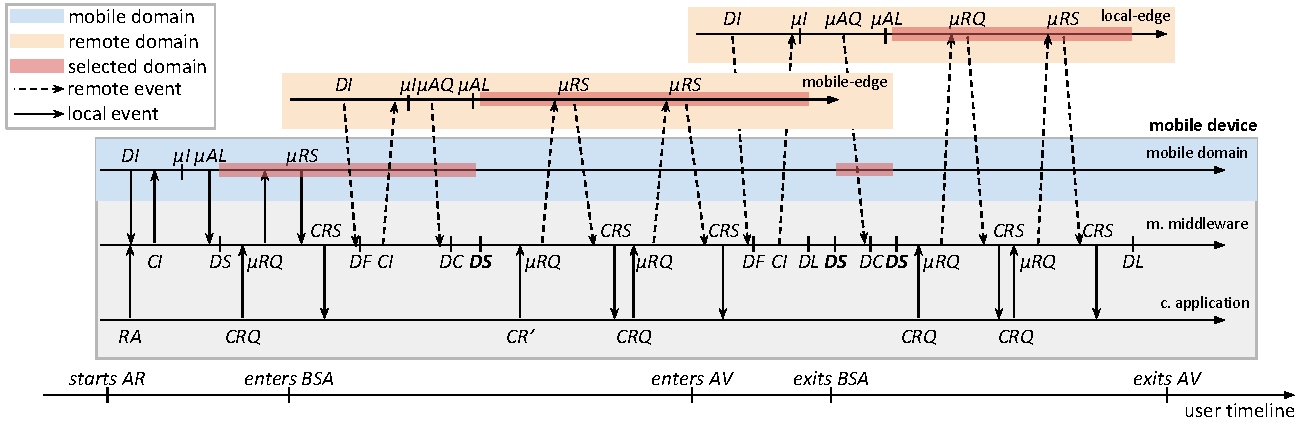
\includegraphics[width=0.95\textwidth]{figs/A3-E-instance-events}
%	\setlength{\belowcaptionskip}{-10pt}
	\caption{A timeline of events from the Running Example scenario (Sec.~\ref{sub:example}). Labels: \textit{domain identification} ($DI$); \textit{$\mu$-service identified} ($\mu I$); \textit{$\mu$-service acquired} ($\mu AQ$); \textit{$\mu$-service allocated} ($\mu AL$); \textit{domain changed} ($DC$); \textit{C-request arrived} ($CR$'); \textit{$\mu$-service request} ($\mu R$'); textit{$\mu$-service identified} ($\mu R$'') \textit{C-request served} ($CR$''); \textit{domain lost} ($DL$).}
	\label{fig:A3-E-instance-events}
\end{figure}

Figure~\ref{fig:A3-E-instance-events} depicts a timeline of events from our Running Example scenario. The timeline starts with our user initializing the AR after entering the touristic area. The mobile middleware starts with the application and receives a \textit{domain identification} ($DI$) from its mobile domain, to be replied with a \textit{client identification} ($CI$). Following the $\mu$-service identification ($\mu I$), the middleware triggers a \textit{$\mu$-service allocated} ($\mu AL$) once the corresponding functions have been registered. After selecting this domain, the middleware triggers a \textit{domain changed} ($DC$), which allows subsequent \textit{C-request} ($CR$'') events to be handled locally. As our user's device enters a base station area (BSA) featuring a mobile-edge domain, the middleware receives a \textit{domain identification} ($DI$) and repeats the previous handshake procedure. To prevent battery drain, the self-management loop decides for the mobile-edge, triggering a $DC$ once the $\mu AL$ signal arrives. After a long period of engagement with that domain, our user enters the AV featuring a local-edge domain. As this is a first contact with the AR, this domain goes through Acquisition, whose completion is indicated by a \textit{$\mu$-service acquired} ($\mu AQ$). Due to a change of network, the connection with the mobile-edge is lost ($DL$). Preventing service interruption, the middleware momentarily switches back to its mobile domain until a $\mu AL$ signal arrives from the local-edge. Upon a \textit{domain confirmed} event (omitted), it switches domain ($DC$). 

%
%The mobile middleware deals with the following events:
%
%{\small
%	\begin{itemize}[noitemsep,topsep=4pt]
%		
%		\item \textbf{C-Request arrived:} indicates the client application has sent a new request to a continuum $\mu$-service. The event contains the target $\mu$-service reference along with any parameters. The middleware must handle it by invoking the $\mu$-service from the currently selected domain.
%		
%		\item \textbf{Request served:} indicates the arrival of a response from a domain for an invoked service. The middleware must handle it with the triggering of a \textit{C-Request served} event to be handled by the client application.
%		
%		%\item \textbf{C-Request served:} indicates a given C-request has been processed. It contains the original $\mu$-service reference along with any return value(s). The client application is responsible for handling the event.	
%		
%		\item \textbf{Domain changed:} indicates a domain have been selected for a specific $\mu$-service. The middleware must handle it by resuming the invocation of any queued and subsequent C-requests to that domain.
%		
%		\item \textbf{Domain absent:} indicates no domain is available for that specific $\mu$-service. The middleware must react by queuing subsequent C-requests and, in case of latency violation, firing a \textit{C-request failed} event.
%		
%	\end{itemize}
%}%

%TODO [Danilo] requirements must be passed by the application before, otherwise the domain selection would need to happen after the request has been fired
%It also contains continuum requirements that must be taken into account by the middleware in the decision of which 

%Two types of event dictate the end of an engagement: i) the client makes no further requests after a time interval; ii) the client selects another domain; and iii) the domain manager requires the deallocation of the service instance. 

%In all three cases, resources become available in the domain. In the latter case, the client is forced to select another domain.


%In this phase the request has already been provisioned by one or more domains and the client-side middleware (CSM) has already selected a specific domain to make the request. 

%handled and parsed by the client-side middleware (CSM), and . 


%Also, one or more domains must have setup and allocated the requested service for execution and the CSM must have selected a specific domain among all providing the same service. Finally, client's request are sent, processed, received, and returned to the application.

%Current FaaS providers allow functions to be exposed as REST services. The same applies to open source platforms implementing the FaaS model. Finally, different approaches may be used to expose local computation as services in mobile platforms like Android and iOS.

%As an exception, computation provided by mobile devices can be accessed by means of local calls to functions executed by the mobile platform.

%%What: how different policies may be employed by domains and clients throughout A3-E-Process
\subsection{A3-E Process: Domain Policies}\label{sec:A3-E-policies}

\begin{figure}[tbp]
	\raggedright
	\subfloat[Different states of a given edge domain with respect to a given client application; the transitions between states triggered by domain events are guarded by policies that may vary according to the type of domain and the SLA with different applications\label{fig:A3-E-domain}] {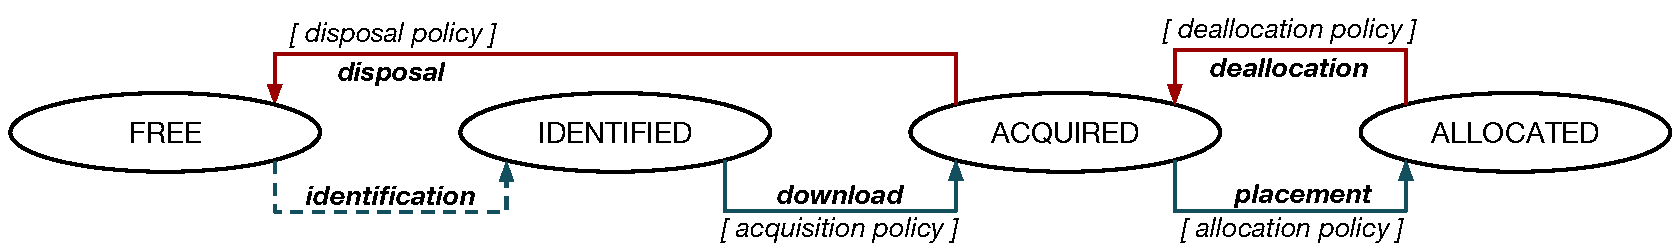
\includegraphics[width=0.95\textwidth]{figs/A3-E-domain}}\hfill
	
	\subfloat[Different states of a given client with respect to a given edge domain; the transitions between states triggered by client events are guarded by policies that may vary according to the client requirements\label{fig:A3-E-client}] {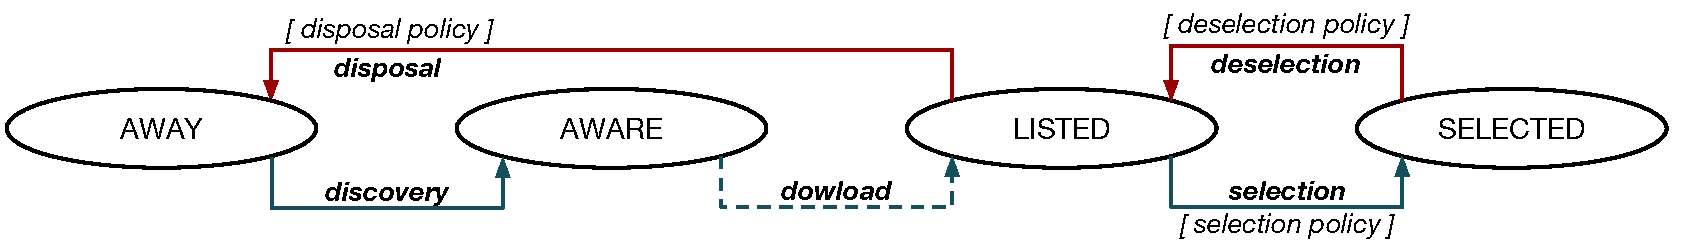
\includegraphics[width=0.95\textwidth]{figs/A3-E-client}}\hfill
	\caption{States and transitions among A3-E phases} \label{fig:A3-E-states}
\end{figure}


%What: the flexibility of A3-E model in terms of policies that regulate the transition among phases

The A3-E process is also flexible with respect to the transitions among subsequent phases. In particular, distinct policies may define different behaviors for the transition. Figures~\ref{fig:A3-E-domain} and~\ref{fig:A3-E-client} depict, respectively, the possible transitions among states of a domain with respect to a client application and vice-versa. Each state is mapped to the corresponding phase in Fig.~\ref{fig:A3-E-model}. 

From the domain perspective, policies affect the following conflicting properties: a) the \textit{efficiency} of domain resource usage; and b) the service setup \textit{delay}. Considering the first request arrival ($FRA$) from a client application as the reference event, the more \textit{reactive} the policies are to that event, the less time domain resources are likely to remain idle before it happens (more efficiency). In contrast, the chances of underutilization and idleness are higher with \textit{proactive} policies (less efficiency). Eq.~\ref{eq:setup_cost} models the total delay of service setup:

\begin{equation}\label{eq:setup_cost}
C_{SETUP} = C_{OFFLINE} + C_{RUNTIME}
\end{equation}

\noindent
in which the first term ($C_{OFFLINE}$) represents the resources required for downloading and installing the services (e.g., network and storage), whilst the later ($C_{RUNTIME}$) represents the resources needed for executing the services (e.g., memory and CPU). 

From the delay point of view, the relation is the opposite: the more \textit{reactive} the policies are with respect to the first request arrival event, the higher the delay the first request to each service is served with. In the other direction, the more \textit{pro-actively} services are made ready for execution, the lower the delay the first request to each of these services is served with. Eq.~\ref{eq:setup_delay} models the total delay of service setup:

%\Delta_{NET} + 
\begin{equation}\label{eq:setup_delay}
L_{SETUP} = \Delta_{AW} + \Delta_{AQ} + \Delta_{AL}
\end{equation}

\noindent
in which the first term ($\Delta_{AW}$) represents the time it takes for clients and domains to become aware of each other. The second term ($\Delta_{AQ}$) represents the time for acquiring all assets of a specific service, whilst the last term ($\Delta_{AL}$) represents the time for allocating resources for the service execution. 

For instance, existing cloud-based FaaS platforms (e.g., Amazon Lambda, Google Cloud Functions, and Apache OpenWhisk) employ on demand allocation of stateless functions, i.e., functions are reactively allocated upon arrival of the first request. Depending on the policy configuration, the platform waits for an idleness interval before deallocating the function~\footnote{\url{https://read.acloud.guru/how-long-does-aws-lambda-keep-your-idle-functions-around-before-a-cold-start-bf715d3b810}}. In these cases, the improved efficiency of the platform in allocating computational resources has the drawback of a setup delay (cold start). 

The domain-side policies in Fig.~\ref{fig:A3-E-domain} can be refined into three types: \textit{proactive} (P), \textit{sequential} (S), and \textit{reactive} (R). 

\begin{itemize}

\item \textbf{Proactive}: acquisition phase starts upon external event preceding the $FR_A$ event (e.g., the prediction of service usage in the near-future). Benefits: first response delay ($FR_D$) does not include $\Delta_{AQ}$. Drawback: acquired artifacts remain idle until usage. Example: stateless functions required by body device applications during a marathon event are fetched the night before the event by mobile-edge domains located along the course. 

\item \textbf{Sequential}: the beginning of acquisition phase is dictated by the completion of the awareness phase. Benefits: service artifacts are only acquired upon detection of a potential client in the domain coverage area, minimizing the likelihood of idleness. Drawbacks: $FR_D$ may include a fraction of $\Delta_{AQ}$ if $FRA$ precedes the end of acquisition. Example: stateless functions to be consumed by a mobile multiplayer game application are acquired by an indoor-edge domain inside a passenger train upon detection of two or more clients in the train.

\item \textbf{Reactive}: acquisition phase starts upon detection of a $FRA$. Benefits: acquisition of service artifacts follows an actual demand, eliminating artifacts storage idleness. Drawbacks: $FR_D$ includes $\Delta_{AQ}$, which may be disruptive for some applications. Example: stateless functions to be consumed by a TODO 

%the notion of a reactive allocation can be extended also to the acquisition of service artifacts. Instead of having functions pre-downloaded and installed, this process could happen in reaction to the first arrival of a request. 

\end{itemize}

In turn, the allocation phase can be triggered according to the following policies:

%The \textit{allocation policies} in Fig.~\ref{fig:A3-E-domain} can be:

\begin{itemize}

\item \textbf{Proactive}: allocation phase starts upon external event preceding the arrival of the first request (e.g., the prediction of service usage in the near-future). Benefits: $FR_D$ does not include $\Delta_{AL}$. Drawback: allocated resources remain idle until $FR_A$. Example: stateless functions to be consumed by connected vehicles are pre-allocated by mobile-edge domains in specific day times.

\item \textbf{Sequential}: allocation phase starts as soon as acquisition phase finishes. Benefits: depends on the acquisition policy. Drawbacks: depends on the acquisition policy. Example: stateless functions required by a marathon application running on body devices are allocated following their acquisition by the mobile-edge domains along the course.

\item \textbf{Reactive}: allocation phase starts as soon as $FR_A$ is detected. Benefits: eliminates idleness by conditioning allocation to an actual service demand. Drawback: $FR_D$ includes $\Delta_{AL}$ (cold start). Example: stateless functions required by a mobile multiplayer game are allocated by a local-edge domain inside a train following the detection of a $FR_A$ event.

\end{itemize}

%
%\begin{itemize}
%	
%	\item \textbf{Proactive}: . Benefits: . Drawback: . Example: .
%	
%	\item \textbf{Reactive}: . Benefits: . Drawback: . Example: .
%	
%\end{itemize}
%
%
%\begin{itemize}
%	
%	\item \textbf{Proactive}: . Benefits: . Drawback: . Example: .
%	
%	\item \textbf{Reactive}: . Benefits: . Drawback: . Example: .
%	
%\end{itemize}
%
%
%\subsubsection{Client-Side Policies}
%
%Clients may also adopt different policies for the selection and deselection of domains (Fig.~\ref{fig:A3-E-client}), namely:
%
%%domains are selected based on their category (cloud, edge, local) or/and 
%
%\begin{itemize}
%	
%	\item \textit{Selection policy}
%	
%	\begin{itemize}
%		
%		\item \textbf{Proactive}: 
%		
%		\item \textbf{Reactive}: 
%		
%	\end{itemize}
%	
%	\item \textit{Deselection policy}
%	
%	\begin{itemize}
%		
%		\item \textbf{Proactive}: 
%		
%		\item \textbf{Reactive}: 
%		
%	\end{itemize}
%\end{itemize}


%
%\subsection{Reference Architecture}
%
%\begin{figure}[tbp]
%	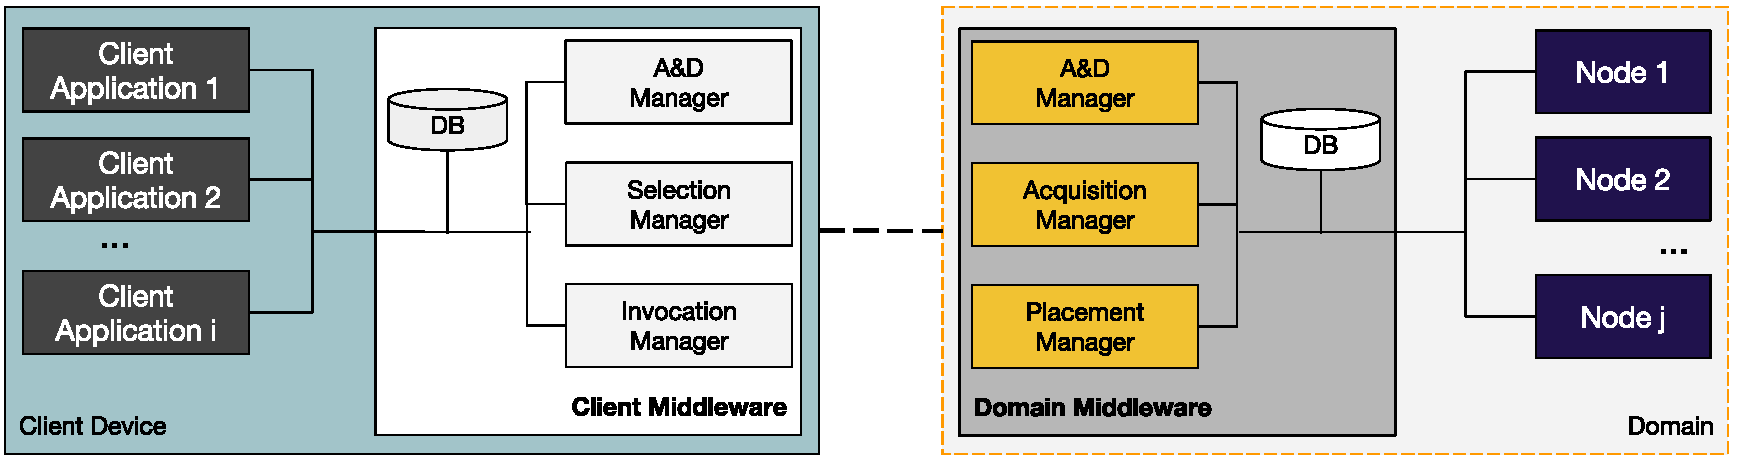
\includegraphics[width=.95\textwidth]{figs/A3-E-reference-architecture}
%	\caption{A3-E architecture in Mobile Devices and edge domains}
%	\label{fig:reference-architecture}
%	\end{figure}

\section{Experimental Evaluation}\label{sec:evaluation}

\subsection{Domains Setup}

%\subsubsection{Domains}

\begin{table}
	\caption{Continuum Setup for the Experimental Evaluation}
	\label{tab:domain-exp-config}
	\begin{tabular*}{1\textwidth}{@{\extracolsep{\fill}}>{\raggedright}p{1.5cm}>{\raggedright}p{6cm}>{\raggedright}p{6cm}}
		\toprule 
		Domain & Machine Resources & Execution Environment\tabularnewline
		\midrule
		\midrule 
		Edge-Local & ubuntu/trusty64-2, 4x vCPUs, 4Gb RAM & Openwhisk, 256 Mb/Action, Python 2.7 + OpenCV \tabularnewline
		\midrule 
		Edge-Mobile & ubuntu/trusty64-2, 8x vCPUs, 16Gb RAM & Openwhisk, 256 Mb/Action, Python 2.7 + OpenCV \tabularnewline
		\midrule 
		Cloud-FaaS & N/A & AWS Lambda, 256 Mb/Function, Python 2.7 + OpenCV \tabularnewline
		\midrule 
		Cloud-IaaS & Autos Scaling Group with t2.micro instances + Amazon Linux AMI 2017  & NodeJs 6.11 server + Python 2.7 + OpenCv \tabularnewline
		\bottomrule
	\end{tabular*}
\end{table}

Table~\ref{tab:domain-exp-config} shows the different domains that were deployed to materialize the computational continuum for the experiments. Edge domains feature the Apache Openwhisk (formerly IBM Openwhisk) serverless framework\footnote{https://openwhisk.incubator.apache.org/} that manages {\em actions} (equivalent to functions). Being open-source, openwhisk is (to date) the only serverless alternative among the major vendors that can be deployed locally or on private clouds. 
%Particularly, openwhisk provides a built-in noSQL database: CouchDB, which is associated with the implemented actions through user-defined triggers and rules. 
Particularly, Edge-local domain is always placed close to the client applications/devices (one or two network hops). This deployment allows us to represent a situation where latency is close to zero, but the computational resources are highly constrained, as scaling-up is not possible due to inherent physical restrictions of the underlying infrastructure. Similarly, the Edge-mobile domain is placed on an university server, where the computational resources are less constrained, and still low latency can be achieved due to physical proximity and data locality. Note that in both cases the domains are deployed in the same LAN that originates the requests, to emulate the few-hop scenario in which devices are directly connected to their nearest Edge domains.


%In this experiment, we considered two alternatives for deploying the serverless continuum architecture, mimicking the behavior of both an edge node and a fog node (Figure~\ref{fig:exp-edge}).  

%The client application is embedded in the edge node, consisting on the postman requests and the node.js endpoint (Figure~\ref{fig:exp-setup1}). 
%On the edge-local alternative, we used a virtual machine running locally, on a regular laptop, with 4x CPU, 4x Gb of RAM and 40 Gb SSD of storage. 

%For the Fog alternative, we deployed the serverless architecture on Policloud\footnote{http://policloud.polimi.it/}, the private IaaS solution of Politecnico di Milano. Here, the computational resources are less constrained, and still low latency can be achieved due to physical proximity (two hops from the client) and data locality. This setup runs on a small cluster of 4 virtual machines with 2x CPU, 4x Gb of Ram and 100 GB SSD, each running a different component of openwhisk (triggers and storage, Http server, controller, and invokers, respectively). Note that in this case the fog node is deployed in the same LAN that originates the requests, to emulate the few-hop scenario in which devices are directly connected to their corresponding MEC.

The serverless cloud alternative (Cloud-FaaS) for this experiment uses AWS Lambda\footnote{https://aws.amazon.com/lambda/} as the first-available and most mature serverless solution in the market. The functions and associated libraries and services (storage, image recognition) are hosted in the same region, which is enforced by AWS to guarantee a certain degree of data locality. Finally, we also deployed the feature recognition functionality as a ``serverful'' Cloud setup (Cloud-IaaS). However, the main goal of this experiment is not to compare traditional cloud services against a serverless solution, but to demonstrate that the proposed continuum can outperform the Cloud under certain circumstances and requirements.


\subsection{Domain Latency Evaluation} 

In order to compare the latency along the continuum, we performed experiments with different number of parallel requests firing at a constant rate. Each request consisted on feature extraction and matching from a sample image. This experiment was performed without using the A3-E middleware, since it aims to evaluate only the different domains.

Figure~\ref{fig:exp-setup1} shows the experimental setup. Capturing and uploading an image is emulated using Postman\footnote{https://www.getpostman.com/}, a JavaScript open source application designed to load test functional behaviors and measure the performance of Web APIs. The  payload for this experiment was a sample image of approximately 65 Kb, which is a reasonable size for this use case considering the requirements regarding low-latency, computation time and battery consumption~\cite{rodriguez16mobile}. 

Then, the image is sent through HTTP/POST and different subsequent steps are executed depending on the domain: Openwhisk actions for both Edge domains, AWS Lambda functions for Cloud-FaaS domain, and a simple Nodejs server that calls a Python function for Cloud-IaaS domain.

%In our edge domains for the experiment, uploading an image to CouchDB (Step 3.a) triggers the action that performs the feature extraction and matching (Step 4.a)  with the points-of-interest, supported by the OpenCV\footnote{\url{http://opencv.org}} visual recognition library (Step 5.a). 


\begin{figure}
	
	\centering
	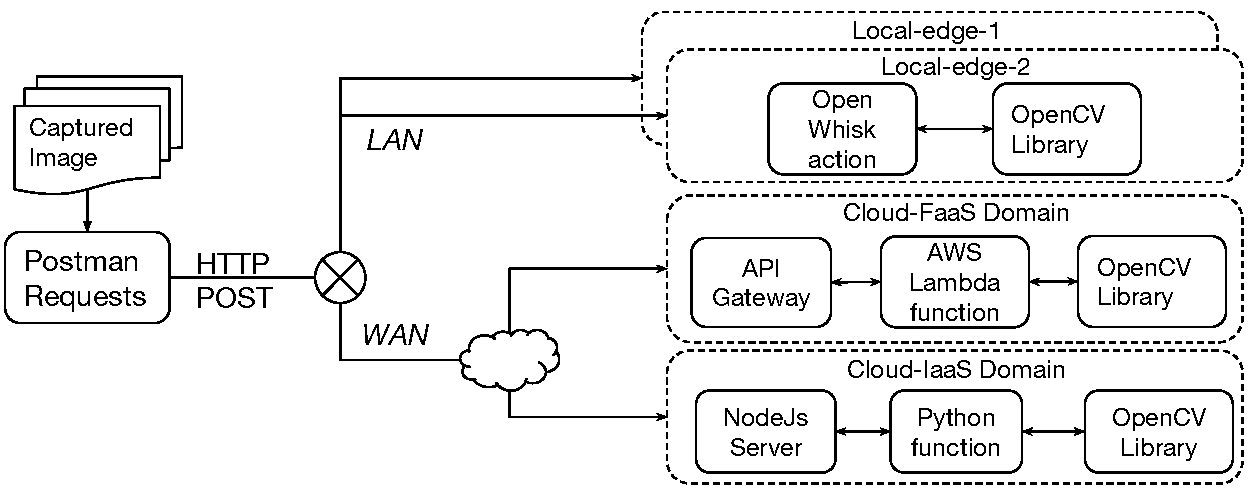
\includegraphics[width=0.9\textwidth]{figs/experimental-setup.pdf}
	\caption{Setup for Latency Experiments}
	\label{fig:exp-setup1}
\end{figure}

%\subsubsection{Baseline Latency}

To measure the latency, the workload was parameterized using different number of parallel clients, which perform 100 requests each, fired at a constant rate of two per second. This setup considers not only the default maximum for concurrent executions in AWS Lambda\footnote{http://docs.aws.amazon.com/lambda/latest/dg/concurrent-executions.html} and Openwhisk\footnote{https://github.com/apache/incubator-openwhisk/blob/master/docs/reference.md}, but also the limited resources of the edge domains. 

The experiment stresses progressively the different domains, and allows to compare the relative latency under each workload. Figure~\ref{fig:latency-domains} shows the average latency for each scenario, averaged through 5 executions. Note that the function computation time (light gray) is distinguished from the overhead (dark gray), which includes network communication (routing, forwarding) and queuing time (when no resources are available to process the request immediately). 

\begin{figure}
	
	\centering
	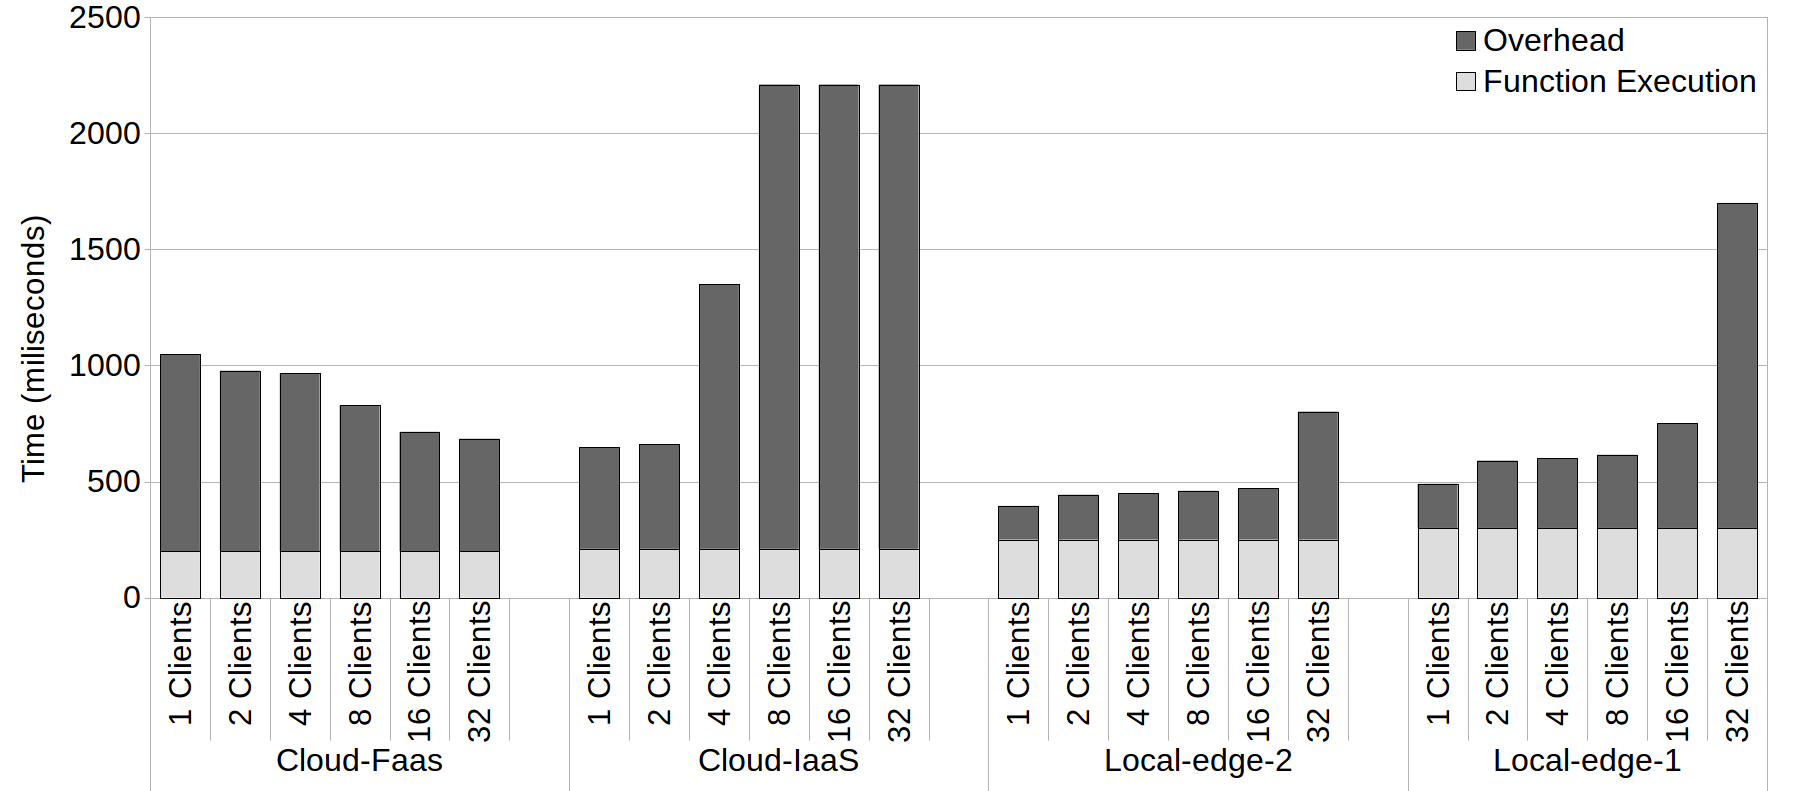
\includegraphics[width=1\textwidth]{figs/latency-domains}
	\caption{Latency results for each domain and different number of clients.}
	\label{fig:latency-domains}
\end{figure}

 For these scenarios, the latency added by the edge domains is less than the latency in both cloud alternatives, considering up to 16 simultaneous clients, with a rate of 2 $requests/second$ each. Regarding the serverless cloud alternative, the overhead reduction is up to 90\% for edge-local and up to 82\% for edge-mobile respectively. Regarding the traditional cloud domain, reductions are up to 77\% and 58\% respectively. Since a scaling-up action triggers when more than one VM instance is needed to handle the workload (that can demand several seconds~\cite{Quatrocchi2016discrete}), requests timeout in the meantime. 
 
 For light to medium workloads, the edge-local and edge-mobile domains outperformed all the other alternatives for this scenario. However, edge-local domain is the most resource-constrained, which hinders its availability under heavier workloads. Interestingly, the traditional cloud domain also outperformed the serverless one (46\% less latency) for light workloads. This can be due to the additional steps performed by the API Gateway in order to forward RESTful calls to lambda functions\footnote{http://docs.aws.amazon.com/lambda/latest/dg/with-on-demand-https.html}. Nevertheless, this advantage is mitigated by the fact that the serverless alternative is more reactive against bursts of workload, scaling faster and offering a fine-grained cost model~\cite{Villamizar2017lambda,Hendrickson:2016}.


%\subsection{Battery} The second set of experiments targeted the measurement of battery consumption of a mobile device in two scenarios: 1) in which feature extraction and matching were performed locally, and 2) these tasks were offloaded to edge servers.

\subsection{Continuum} The next set of experiments targeted the evaluation of A3-E with a computational continuum scenario. In specific, the evaluation consisted of a mobile device hosting a simplified version of an AR application with the feature extraction and matching modeled as stateless functions that can be executed locally (Java Functions), in an edge-based FaaS platform (OpenWhisk), or a cloud-based FaaS platform (Amazon Lambda). We measured the following parameters: Battery consumption, total execution time, and time per call. The experiment featured four different scenarios: With only one domain available (either locally in the device, edge-mobile or cloud-faas), and then with all domains available at the same time (all-domains). \textcolor{blue}{[TODO] (1) Explain the probabilities of having each domain available. (2) Discuss the relevance of the results} 
Figure~\ref{fig:exp-a3e} shows the results for the experiment, averaged among 5 executions for each scenario.

\begin{figure}[tbp]
	\raggedright
	\subfloat[Battery consumption (\%)\label{fig:battery-a3e}] {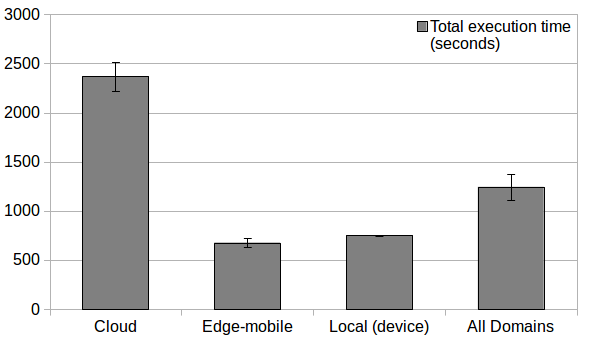
\includegraphics[width=0.5\textwidth]{figs/total-exec-time-A3E}}
	\subfloat[Total execution time (seconds)\label{fig:total-exec-a3e}] {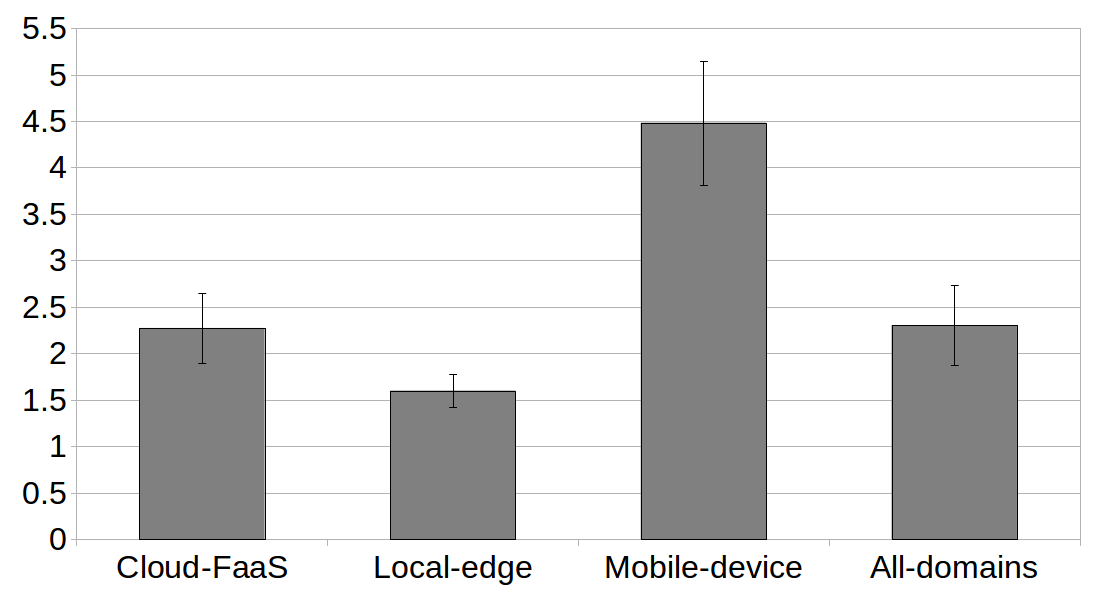
\includegraphics[width=0.5\textwidth]{figs/battery-consumption-A3E}}
	
	\centering\subfloat[Execution time per call (miliseconds)\label{fig:time-per-call-a3e}] {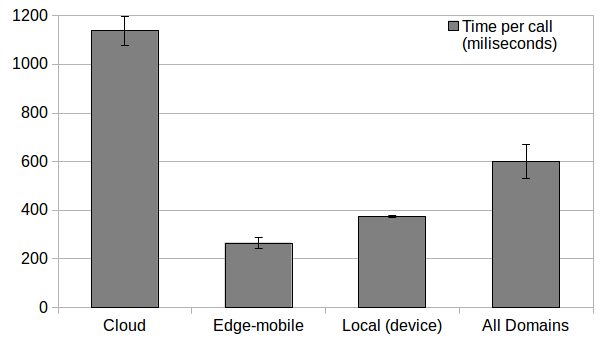
\includegraphics[width=0.5\textwidth]{figs/time-per-call-A3E}}

	\caption{A3-E experimental evaluation results} \label{fig:exp-a3e}
\end{figure}






\section{Conclusions and Future Work}\label{sec:conclusions}

%Due to its particular characteristics, which inherit and complement those of serverless computing, A3-E provides a suitable model for the realization of edge computing as part of a  computational continuum composed of cloud, edge, and mobile clients.


\section*{Acknowledgements}

``This work was supported with grant by National Council for Scientific and Technological Development (CNPq) - Brazil''

%\input{samplebody-journals}
\bibliographystyle{ACM-Reference-Format-Journals}
\bibliography{bibliography}


\end{document}
